\documentclass{article}
\usepackage{graphicx}
\usepackage{geometry}
\usepackage{hyperref}
\usepackage{booktabs}
\usepackage{subcaption}
\usepackage{amsmath}

\geometry{
    a4paper,
    margin=0.6in
}

\hypersetup{
    colorlinks=true,
    linkcolor=blue,
    filecolor=magenta,      
    urlcolor=cyan,
}

\title{SNN Surrogate Gradient Parameter Comparison:\\ArcTangent ($\alpha$) vs. Triangular ($\beta$) vs. Box ($\beta$) under Robust Sweeps}
\author{ByzFL SNN Benchmark}
\date{\today}

\begin{document}

\maketitle

\section{Introduction}
This document presents a comprehensive comparison of Spiking Neural Network (SNN) robustness on the MNIST dataset under data heterogeneity ($\gamma$) and Byzantine attacks ($f$). We evaluate and compare three surrogate gradient functions under fixed attacks and overall:
\begin{itemize}
    \item \textbf{ArcTangent (\texttt{atan})}: parameterized by stiffness factor $\alpha \in \{0.5, 0.75, 1.0, 1.5, 2.0\}$.
    \item \textbf{Triangular (\texttt{tri})}: parameterized by stiffness factor $\beta \in \{0.5, 0.75, 1.0, 1.25, 1.5, 2.0\}$.
    \item \textbf{Box (\texttt{box})}: parameterized by stiffness factor $\beta \in \{0.25, 0.5, 0.75, 1.0, 1.25, 2.0\}$.
\end{itemize}

The evaluations are carried out on $N = 10$ honest nodes + $f$ Byzantine nodes (up to $f=5$ for \texttt{atan}, \texttt{tri}, and \texttt{box}), across non-IID levels $\gamma \in \{1.0, 0.66, 0.33, 0.0\}$. 

The heatmaps display the best test accuracy at convergence (validation-based best step) achieved by the optimal aggregator choice (Centered Clipping or Geometric Median, with NNM and ARC pre-aggregation). We evaluate performance under three scenarios:
\begin{enumerate}
    \item \textbf{Best Overall Aggregator (Worst-Case Across Attacks)}
    \item \textbf{Optimal A Little Is Enough (ALIE) Attack} (\texttt{Optimal\_ALittleIsEnough\_neg1})
    \item \textbf{Sign Flipping (SF) Attack} (\texttt{SignFlipping})
\end{enumerate}

\clearpage

\section{ArcTangent (\texttt{atan}) Surrogate Gradient stiffness sweeps}

\subsection{Best Overall Aggregator (Worst-Case Across Attacks)}
The figure below displays the test accuracy heatmaps under the worst-case attack scenario for different $\alpha$ values of the ArcTangent surrogate gradient.

\begin{figure}[htbp]
    \centering
    \begin{subfigure}[b]{0.32\textwidth}
        \centering
        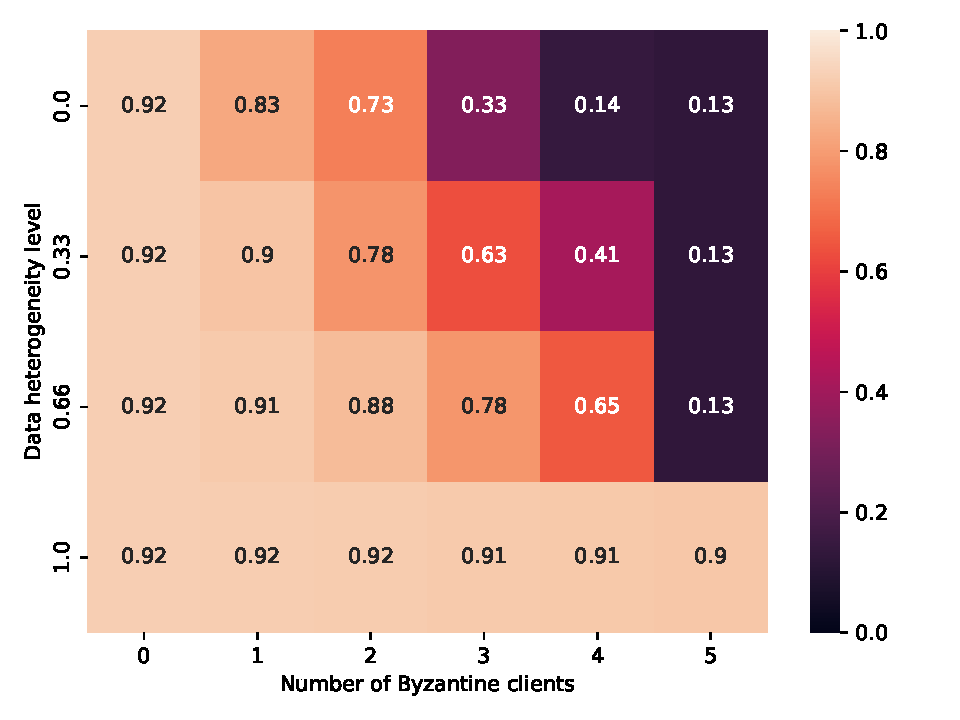
\includegraphics[width=\textwidth]{heatmap_alpha_0_5_best.pdf}
        \caption{$\alpha = 0.5$}
        \label{fig:alpha_0_5_best}
    \end{subfigure}
    \hfill
    \begin{subfigure}[b]{0.32\textwidth}
        \centering
        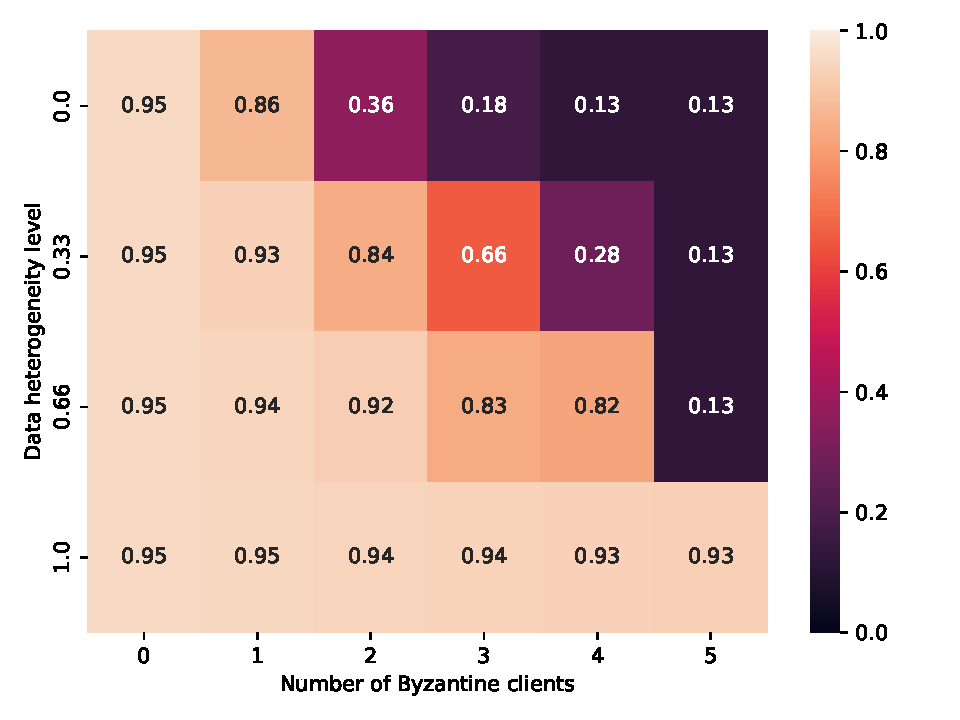
\includegraphics[width=\textwidth]{heatmap_alpha_0_75_best.pdf}
        \caption{$\alpha = 0.75$}
        \label{fig:alpha_0_75_best}
    \end{subfigure}
    \hfill
    \begin{subfigure}[b]{0.32\textwidth}
        \centering
        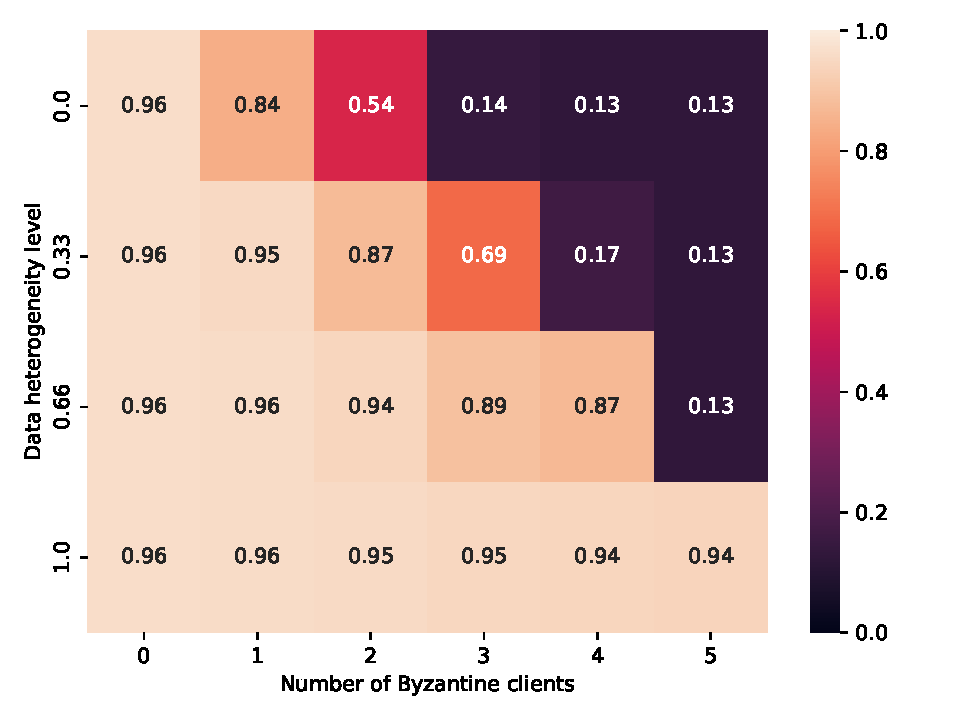
\includegraphics[width=\textwidth]{heatmap_alpha_1_0_best.pdf}
        \caption{$\alpha = 1.0$}
        \label{fig:alpha_1_0_best}
    \end{subfigure}
    
    \vspace{0.4cm}
    
    \begin{subfigure}[b]{0.32\textwidth}
        \centering
        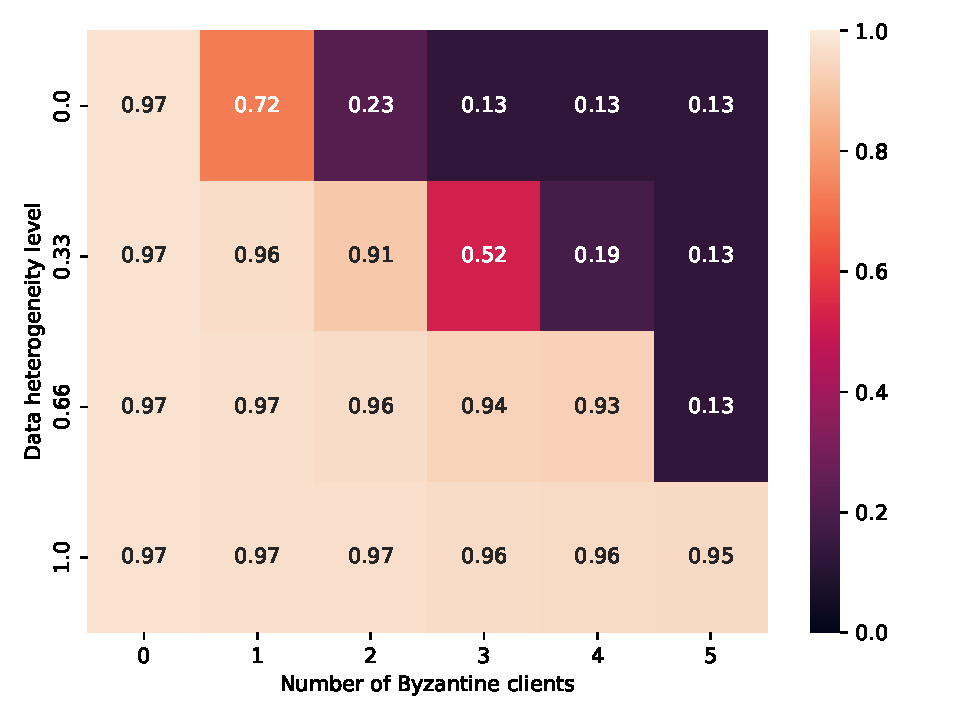
\includegraphics[width=\textwidth]{heatmap_alpha_1_5_best.pdf}
        \caption{$\alpha = 1.5$}
        \label{fig:alpha_1_5_best}
    \end{subfigure}
    \hfill
    \begin{subfigure}[b]{0.32\textwidth}
        \centering
        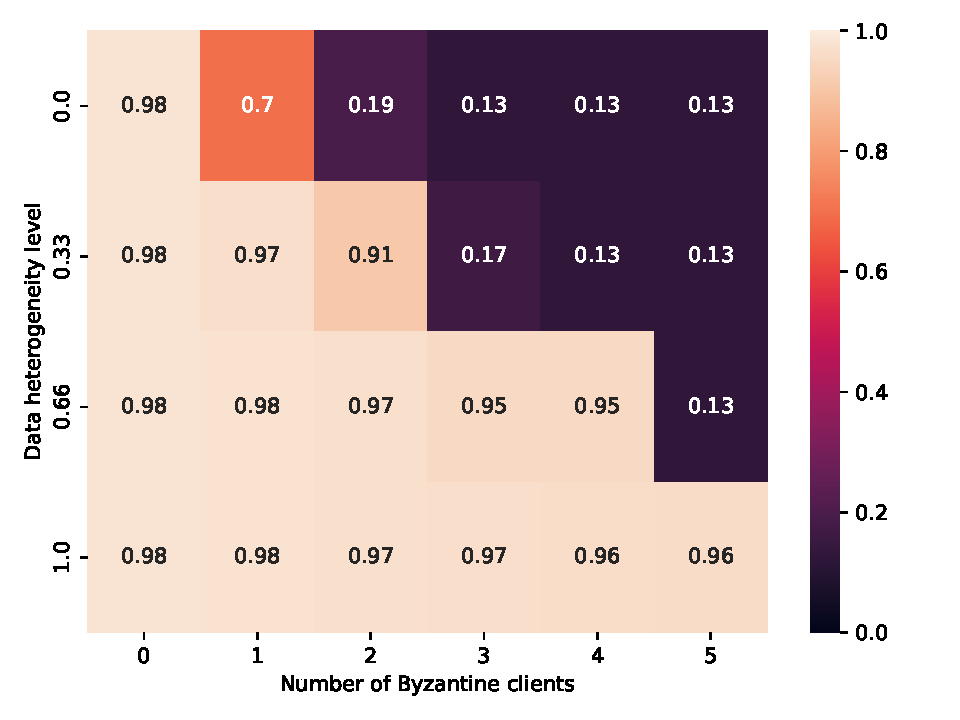
\includegraphics[width=\textwidth]{heatmap_alpha_2_0_best.pdf}
        \caption{$\alpha = 2.0$}
        \label{fig:alpha_2_0_best}
    \end{subfigure}
    \hfill
    \begin{subfigure}[b]{0.32\textwidth}
        \centering
        \vspace{2cm}
        \label{fig:alpha_spacer_best}
    \end{subfigure}
    
    \caption{ArcTangent (\texttt{atan}) comparison for best overall aggregator (worst-case) for $\alpha \in \{0.5, 0.75, 1.0, 1.5, 2.0\}$.}
    \label{fig:atan_comparison_best}
\end{figure}

\clearpage

\subsection{Optimal ALIE Attack}
The figure below displays the best test accuracy heatmaps under the Optimal ALIE attack for different $\alpha$ values of the ArcTangent surrogate gradient.

\begin{figure}[htbp]
    \centering
    \begin{subfigure}[b]{0.32\textwidth}
        \centering
        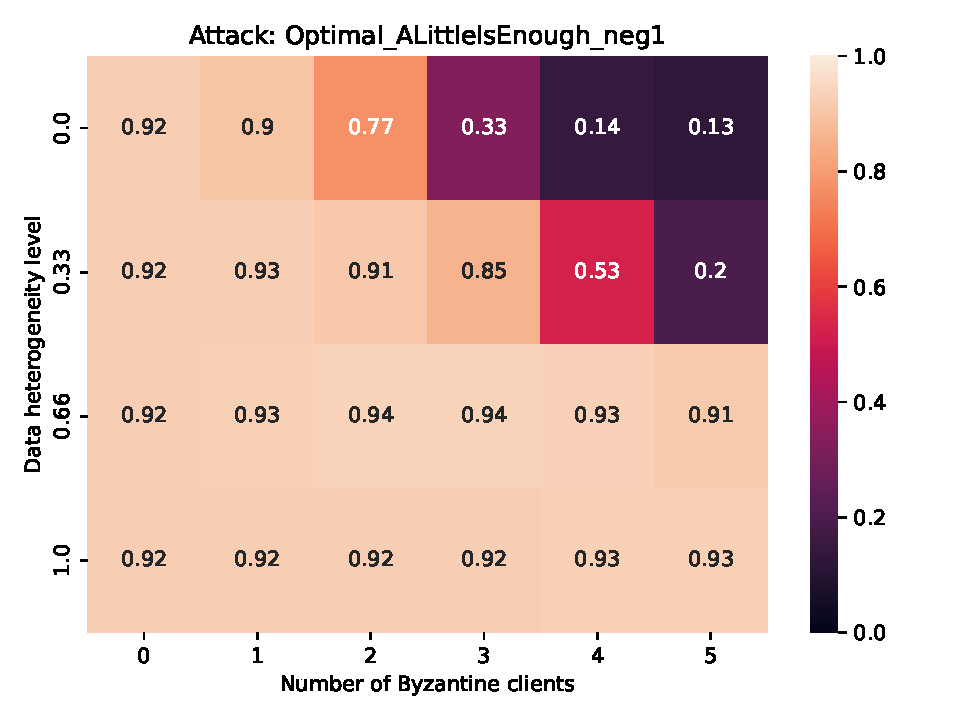
\includegraphics[width=\textwidth]{heatmap_alpha_0_5_optalie.pdf}
        \caption{$\alpha = 0.5$}
        \label{fig:alpha_0_5_optalie}
    \end{subfigure}
    \hfill
    \begin{subfigure}[b]{0.32\textwidth}
        \centering
        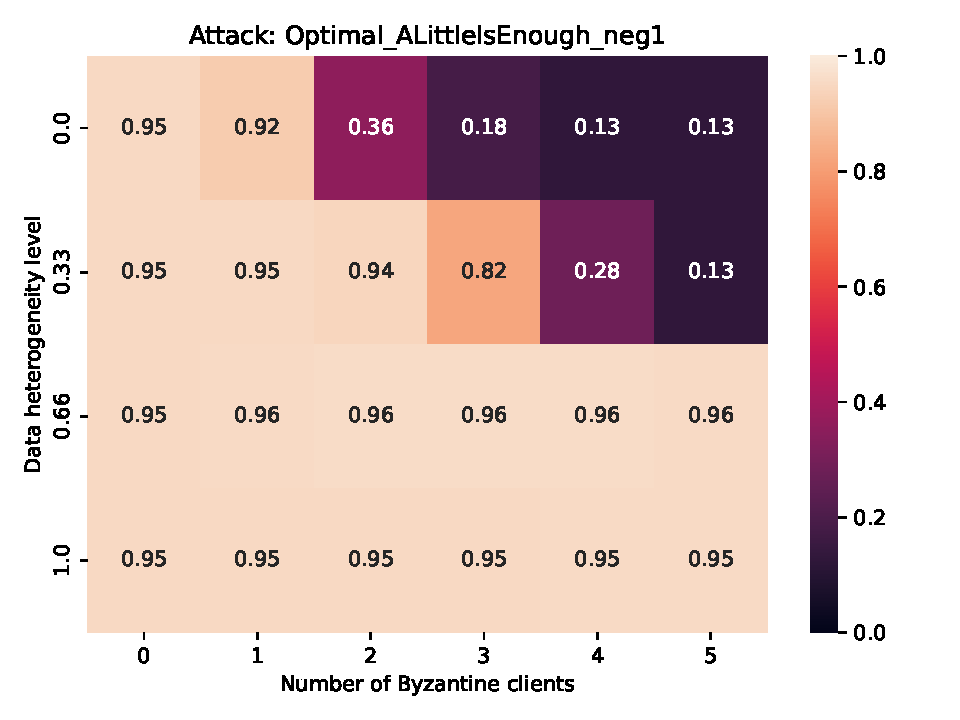
\includegraphics[width=\textwidth]{heatmap_alpha_0_75_optalie.pdf}
        \caption{$\alpha = 0.75$}
        \label{fig:alpha_0_75_optalie}
    \end{subfigure}
    \hfill
    \begin{subfigure}[b]{0.32\textwidth}
        \centering
        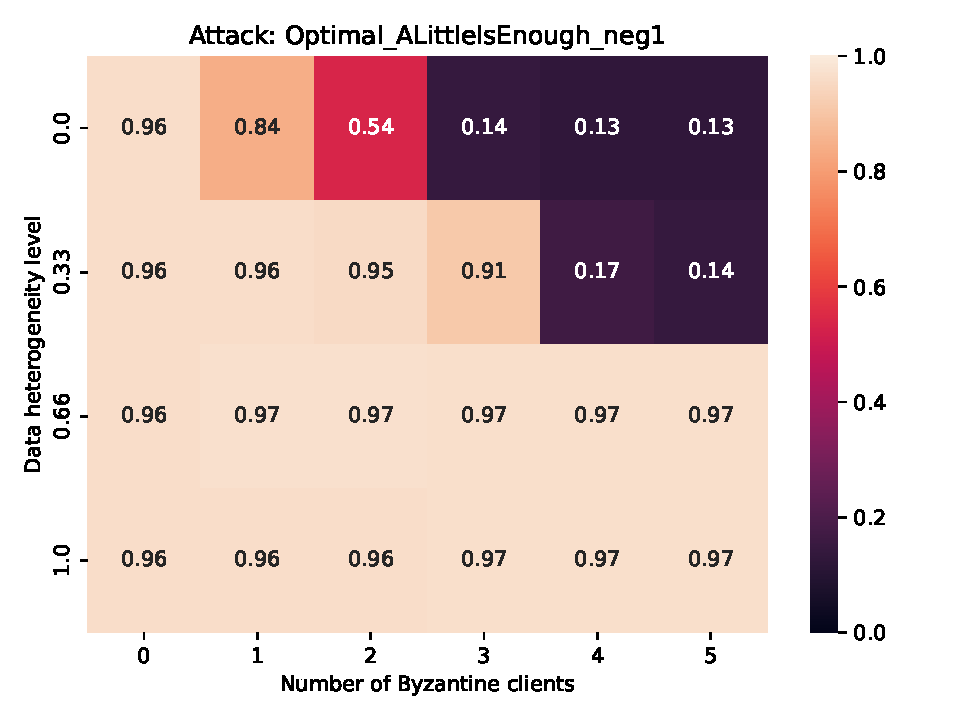
\includegraphics[width=\textwidth]{heatmap_alpha_1_0_optalie.pdf}
        \caption{$\alpha = 1.0$}
        \label{fig:alpha_1_0_optalie}
    \end{subfigure}
    
    \vspace{0.4cm}
    
    \begin{subfigure}[b]{0.32\textwidth}
        \centering
        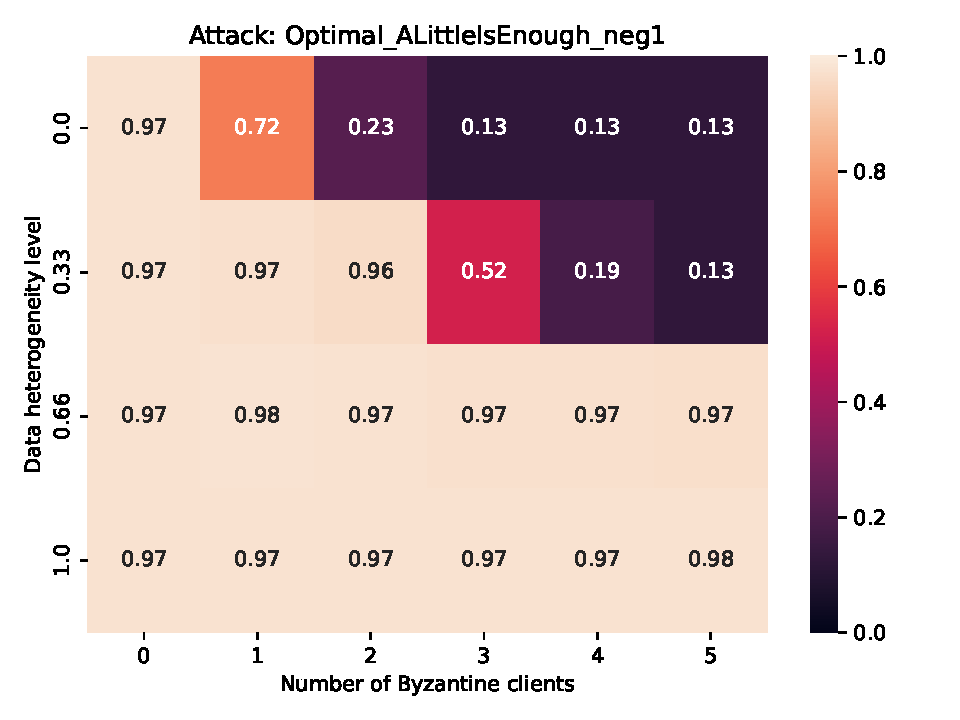
\includegraphics[width=\textwidth]{heatmap_alpha_1_5_optalie.pdf}
        \caption{$\alpha = 1.5$}
        \label{fig:alpha_1_5_optalie}
    \end{subfigure}
    \hfill
    \begin{subfigure}[b]{0.32\textwidth}
        \centering
        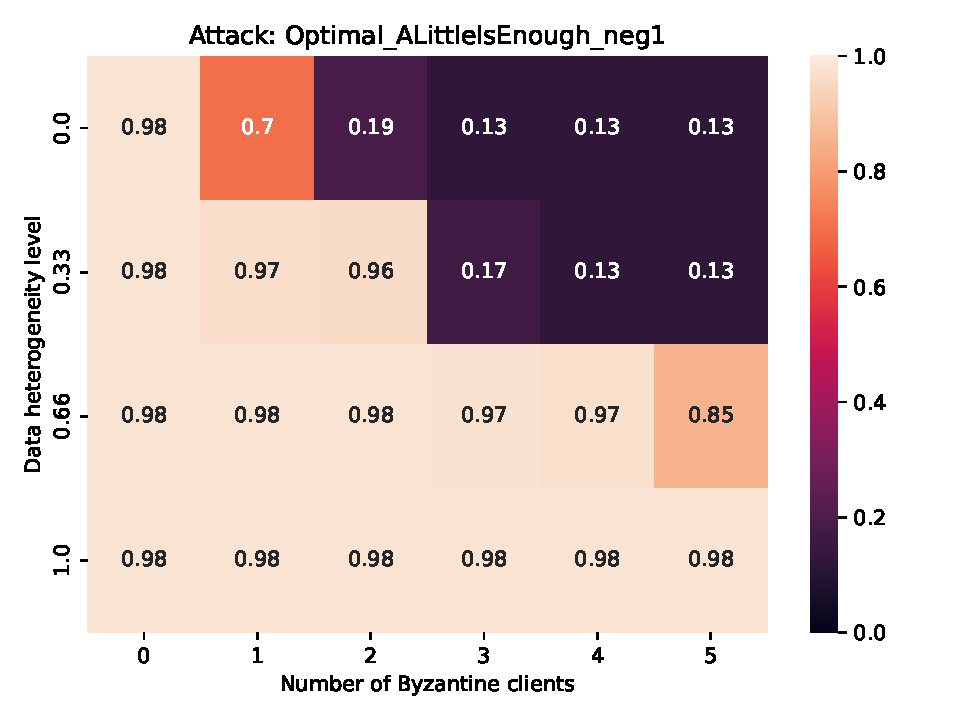
\includegraphics[width=\textwidth]{heatmap_alpha_2_0_optalie.pdf}
        \caption{$\alpha = 2.0$}
        \label{fig:alpha_2_0_optalie}
    \end{subfigure}
    \hfill
    \begin{subfigure}[b]{0.32\textwidth}
        \centering
        \vspace{2cm}
        \label{fig:alpha_spacer_optalie}
    \end{subfigure}
    
    \caption{ArcTangent (\texttt{atan}) comparison under Optimal ALIE attack for $\alpha \in \{0.5, 0.75, 1.0, 1.5, 2.0\}$.}
    \label{fig:atan_comparison_optalie}
\end{figure}

\clearpage

\subsection{Sign Flipping Attack}
The figure below displays the best test accuracy heatmaps under the Sign Flipping attack for different $\alpha$ values of the ArcTangent surrogate gradient.

\begin{figure}[htbp]
    \centering
    \begin{subfigure}[b]{0.32\textwidth}
        \centering
        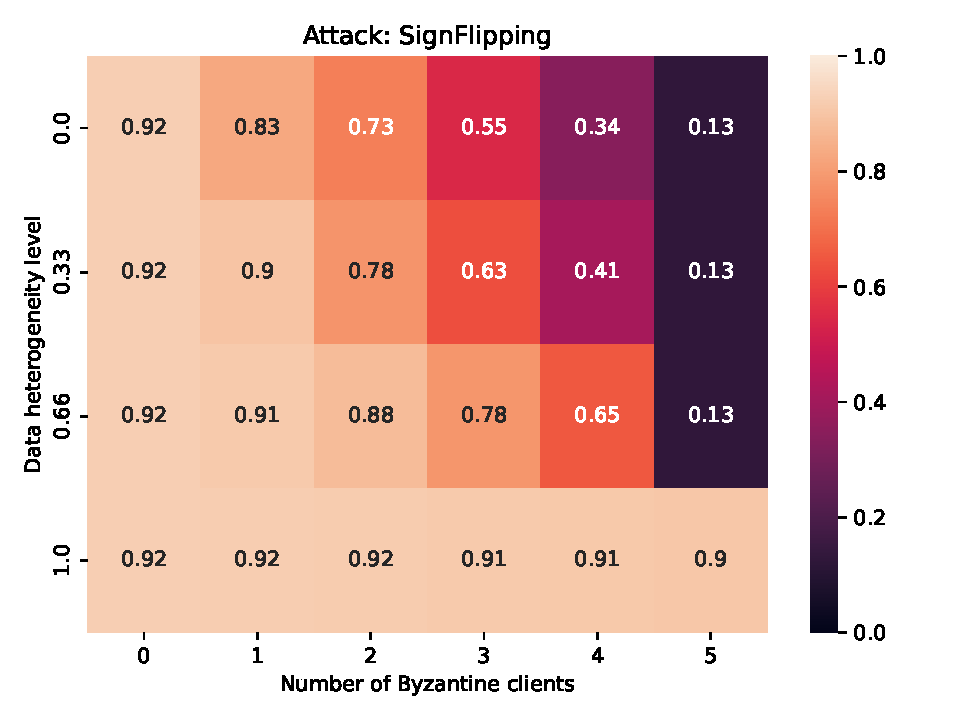
\includegraphics[width=\textwidth]{heatmap_alpha_0_5_sf.pdf}
        \caption{$\alpha = 0.5$}
        \label{fig:alpha_0_5_sf}
    \end{subfigure}
    \hfill
    \begin{subfigure}[b]{0.32\textwidth}
        \centering
        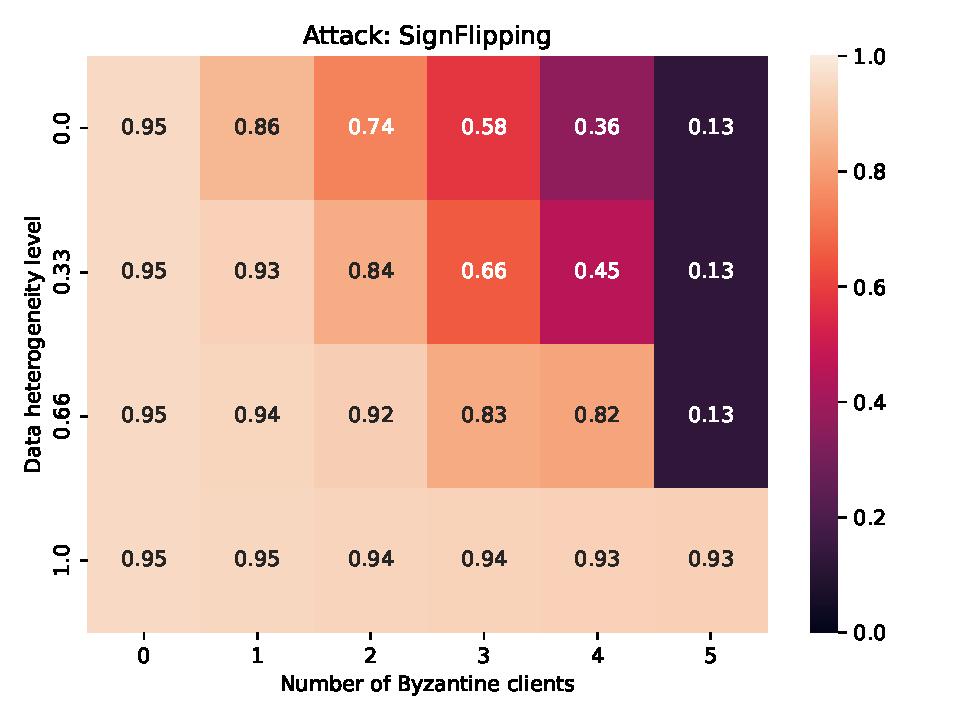
\includegraphics[width=\textwidth]{heatmap_alpha_0_75_sf.pdf}
        \caption{$\alpha = 0.75$}
        \label{fig:alpha_0_75_sf}
    \end{subfigure}
    \hfill
    \begin{subfigure}[b]{0.32\textwidth}
        \centering
        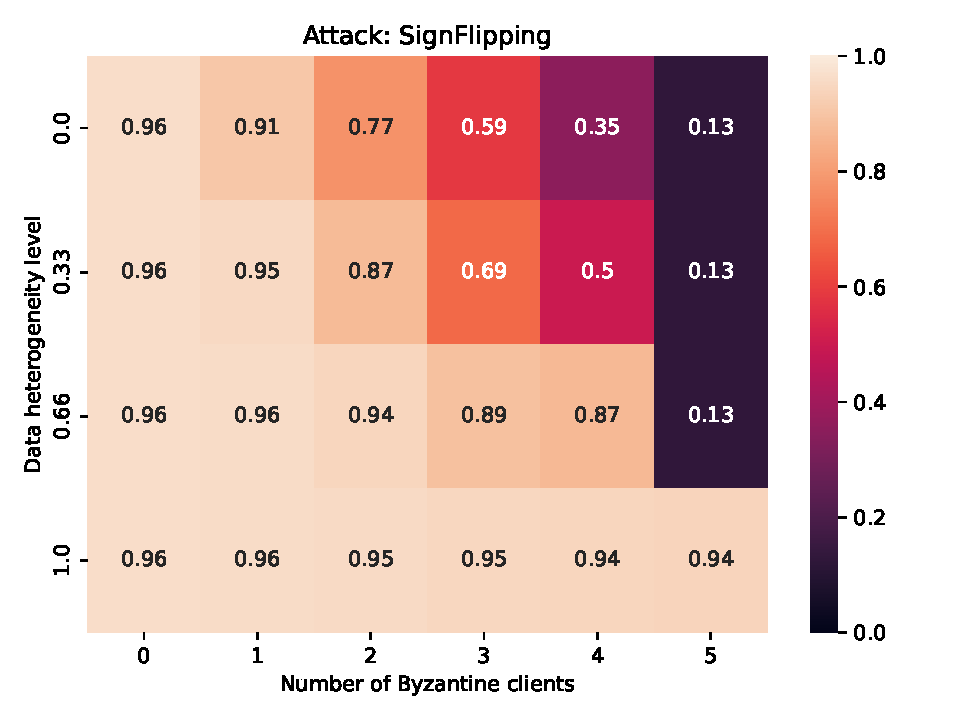
\includegraphics[width=\textwidth]{heatmap_alpha_1_0_sf.pdf}
        \caption{$\alpha = 1.0$}
        \label{fig:alpha_1_0_sf}
    \end{subfigure}
    
    \vspace{0.4cm}
    
    \begin{subfigure}[b]{0.32\textwidth}
        \centering
        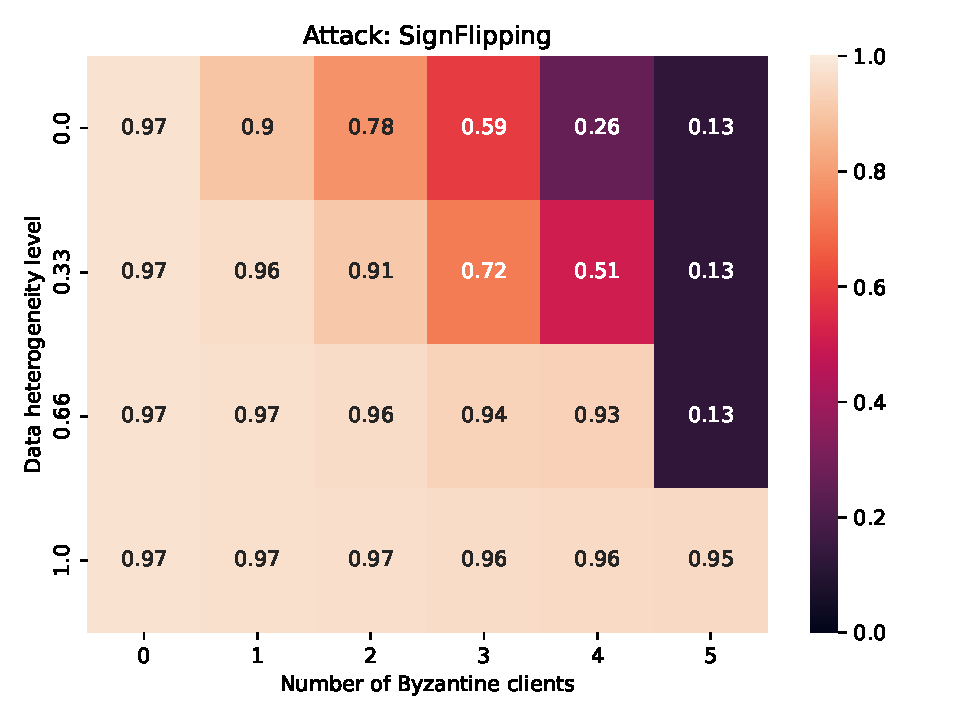
\includegraphics[width=\textwidth]{heatmap_alpha_1_5_sf.pdf}
        \caption{$\alpha = 1.5$}
        \label{fig:alpha_1_5_sf}
    \end{subfigure}
    \hfill
    \begin{subfigure}[b]{0.32\textwidth}
        \centering
        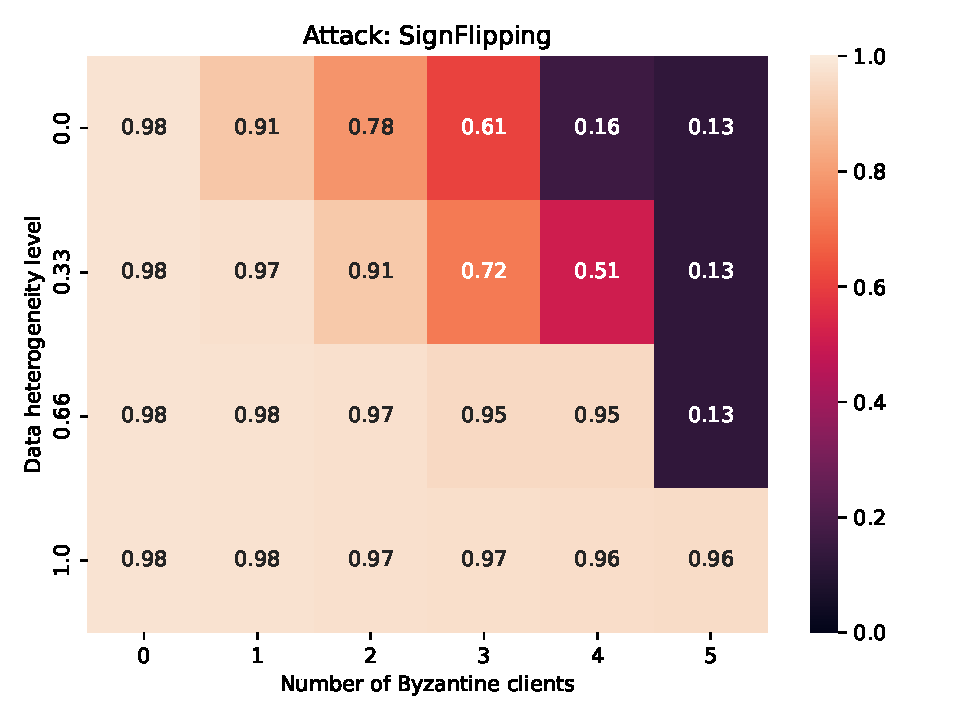
\includegraphics[width=\textwidth]{heatmap_alpha_2_0_sf.pdf}
        \caption{$\alpha = 2.0$}
        \label{fig:alpha_2_0_sf}
    \end{subfigure}
    \hfill
    \begin{subfigure}[b]{0.32\textwidth}
        \centering
        \vspace{2cm}
        \label{fig:alpha_spacer_sf}
    \end{subfigure}
    
    \caption{ArcTangent (\texttt{atan}) comparison under Sign Flipping attack for $\alpha \in \{0.5, 0.75, 1.0, 1.5, 2.0\}$.}
    \label{fig:atan_comparison_sf}
\end{figure}

\clearpage

\section{Triangular (\texttt{tri}) Surrogate Gradient stiffness sweeps}

\subsection{Best Overall Aggregator (Worst-Case Across Attacks)}
The figure below displays the test accuracy heatmaps under the worst-case attack scenario for different $\beta$ values of the Triangular surrogate gradient.

\begin{figure}[htbp]
    \centering
    \begin{subfigure}[b]{0.32\textwidth}
        \centering
        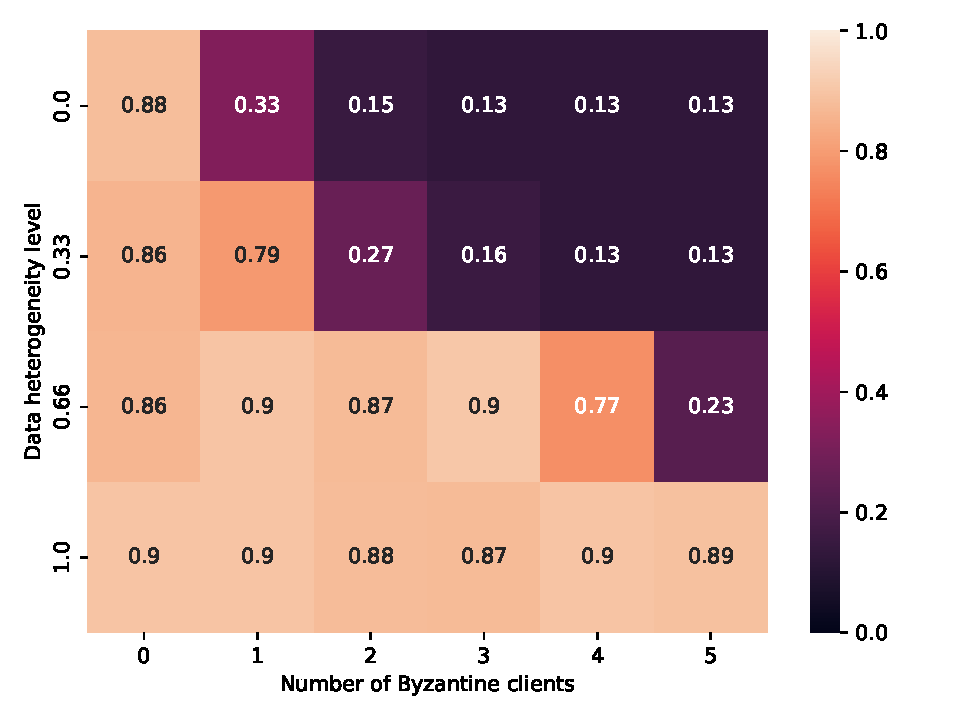
\includegraphics[width=\textwidth]{heatmap_tri_beta_0_5_best.pdf}
        \caption{$\beta = 0.5$}
        \label{fig:beta_0_5_best}
    \end{subfigure}
    \hfill
    \begin{subfigure}[b]{0.32\textwidth}
        \centering
        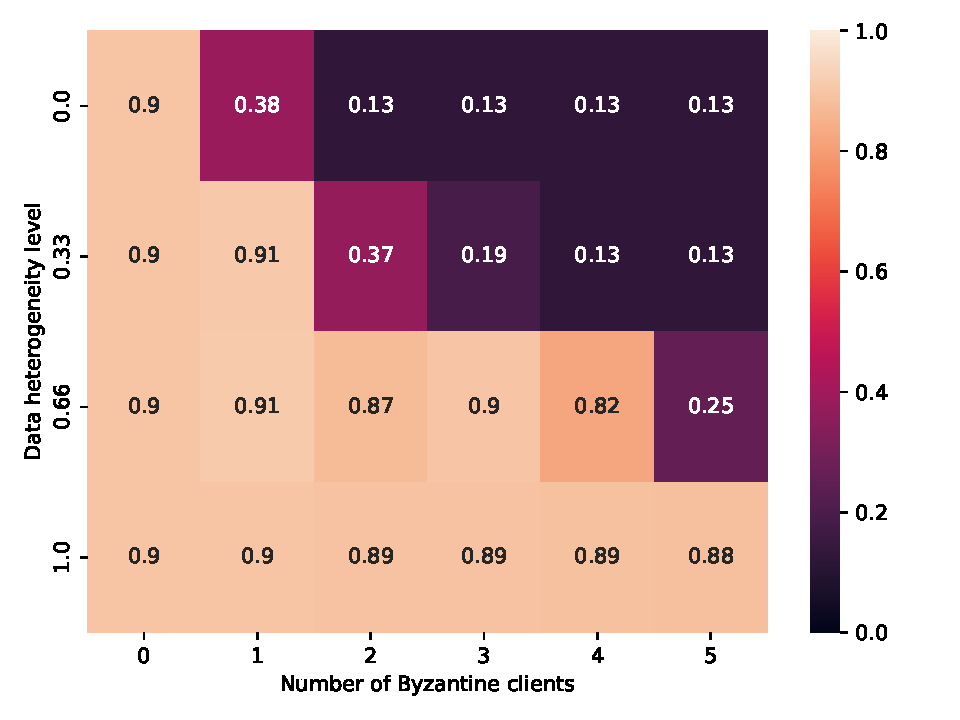
\includegraphics[width=\textwidth]{heatmap_tri_beta_0_75_best.pdf}
        \caption{$\beta = 0.75$}
        \label{fig:beta_0_75_best}
    \end{subfigure}
    \hfill
    \begin{subfigure}[b]{0.32\textwidth}
        \centering
        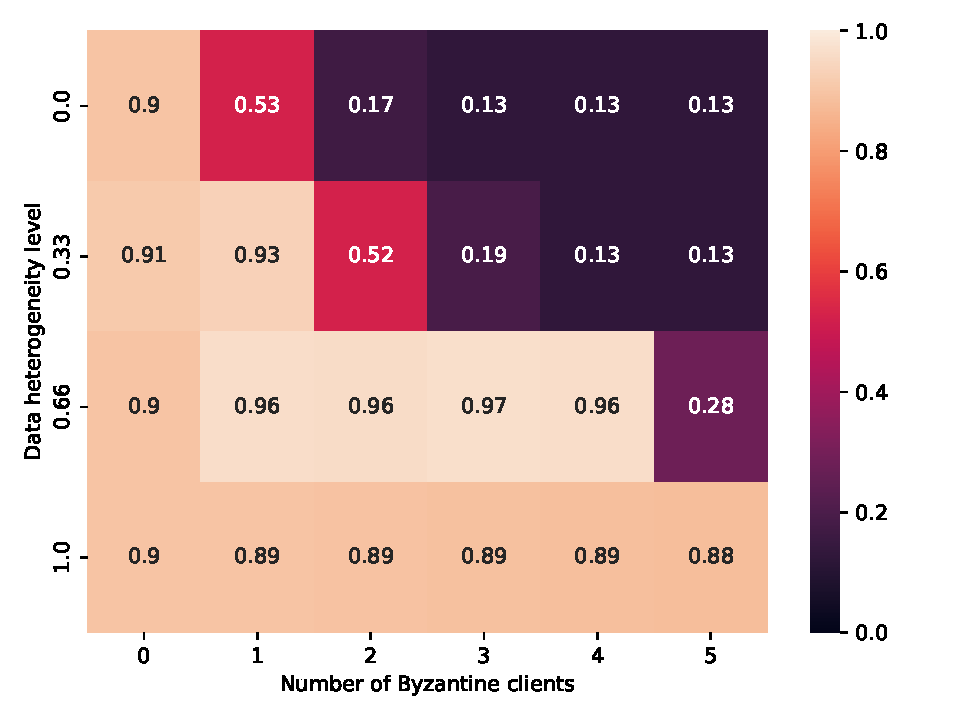
\includegraphics[width=\textwidth]{heatmap_tri_beta_1_0_best.pdf}
        \caption{$\beta = 1.0$}
        \label{fig:beta_1_0_best}
    \end{subfigure}
    
    \vspace{0.4cm}
    
    \begin{subfigure}[b]{0.32\textwidth}
        \centering
        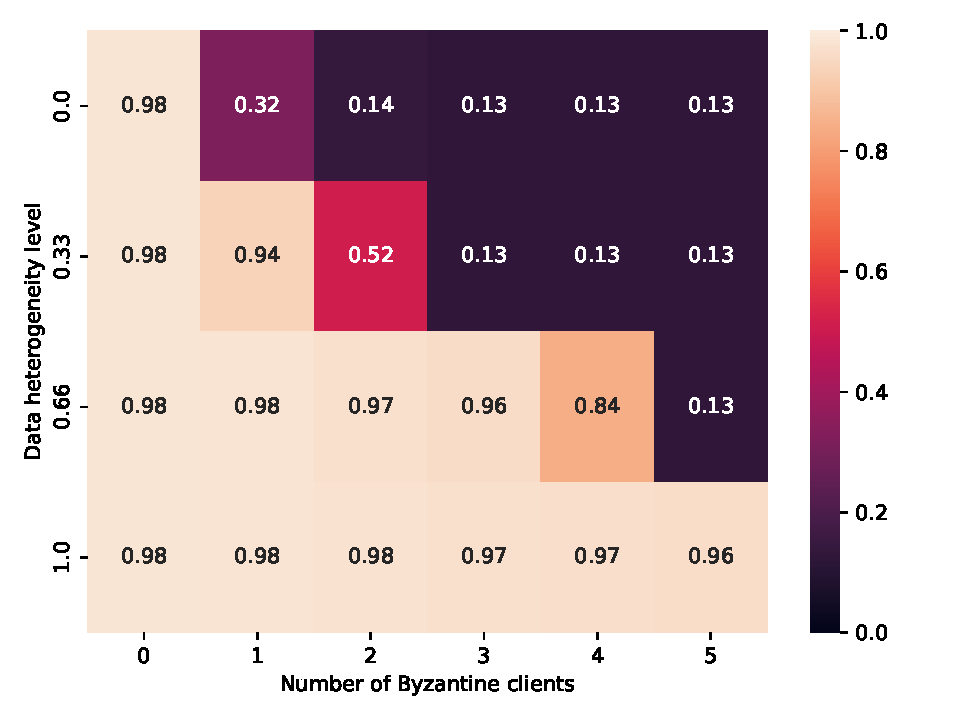
\includegraphics[width=\textwidth]{heatmap_tri_beta_1_25_best.pdf}
        \caption{$\beta = 1.25$}
        \label{fig:beta_1_25_best}
    \end{subfigure}
    \hfill
    \begin{subfigure}[b]{0.32\textwidth}
        \centering
        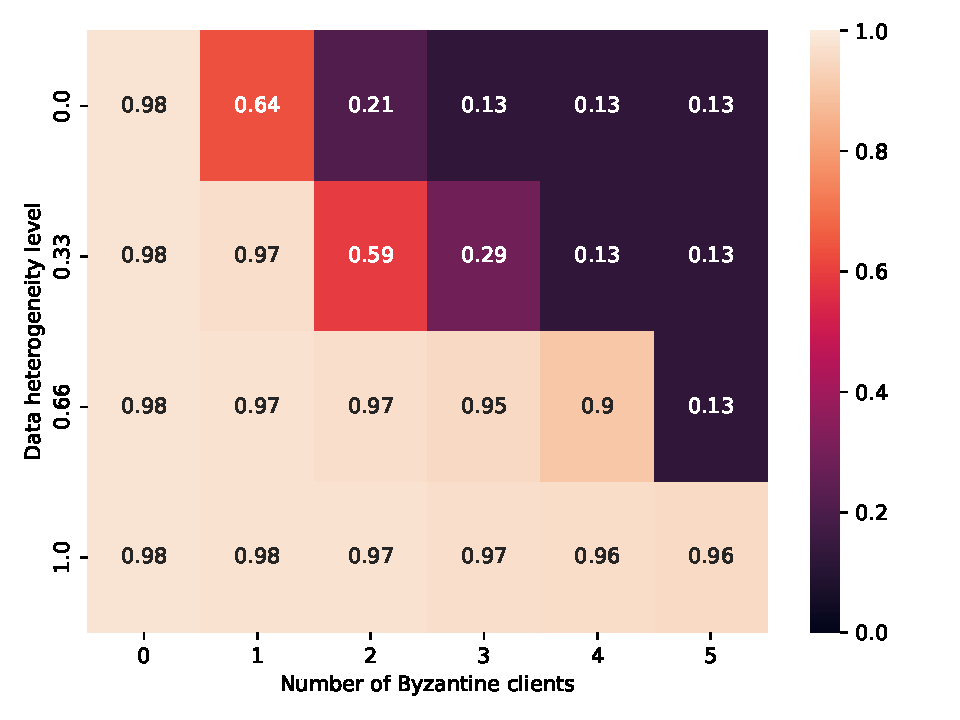
\includegraphics[width=\textwidth]{heatmap_tri_beta_1_5_best.pdf}
        \caption{$\beta = 1.5$}
        \label{fig:beta_1_5_best}
    \end{subfigure}
    \hfill
    \begin{subfigure}[b]{0.32\textwidth}
        \centering
        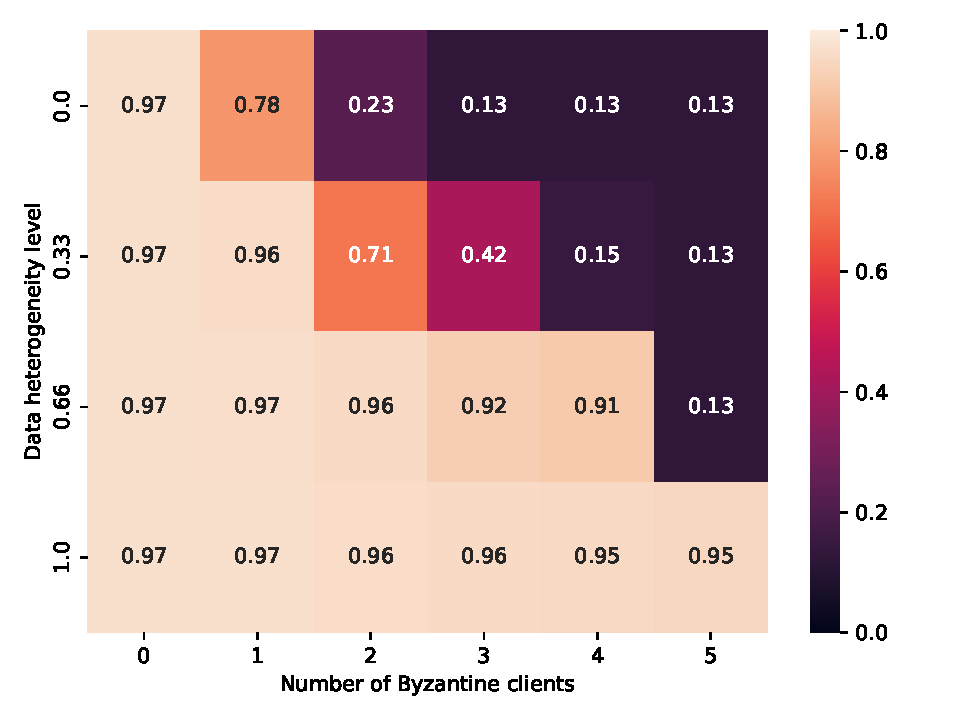
\includegraphics[width=\textwidth]{heatmap_tri_beta_2_0_best.pdf}
        \caption{$\beta = 2.0$}
        \label{fig:beta_2_0_best}
    \end{subfigure}
    
    \caption{Triangular (\texttt{tri}) comparison for best overall aggregator (worst-case) for $\beta \in \{0.5, 0.75, 1.0, 1.25, 1.5, 2.0\}$.}
    \label{fig:tri_comparison_best}
\end{figure}

\clearpage

\subsection{Optimal ALIE Attack}
The figure below displays the best test accuracy heatmaps under the Optimal ALIE attack for different $\beta$ values of the Triangular surrogate gradient.

\begin{figure}[htbp]
    \centering
    \begin{subfigure}[b]{0.32\textwidth}
        \centering
        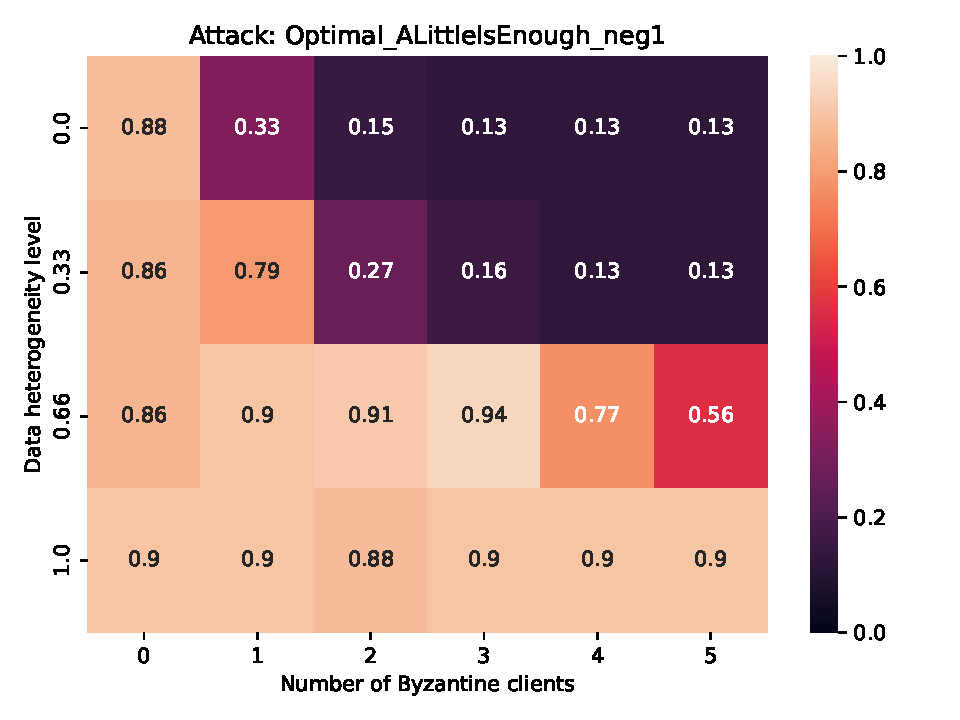
\includegraphics[width=\textwidth]{heatmap_tri_beta_0_5_optalie.pdf}
        \caption{$\beta = 0.5$}
        \label{fig:beta_0_5_optalie}
    \end{subfigure}
    \hfill
    \begin{subfigure}[b]{0.32\textwidth}
        \centering
        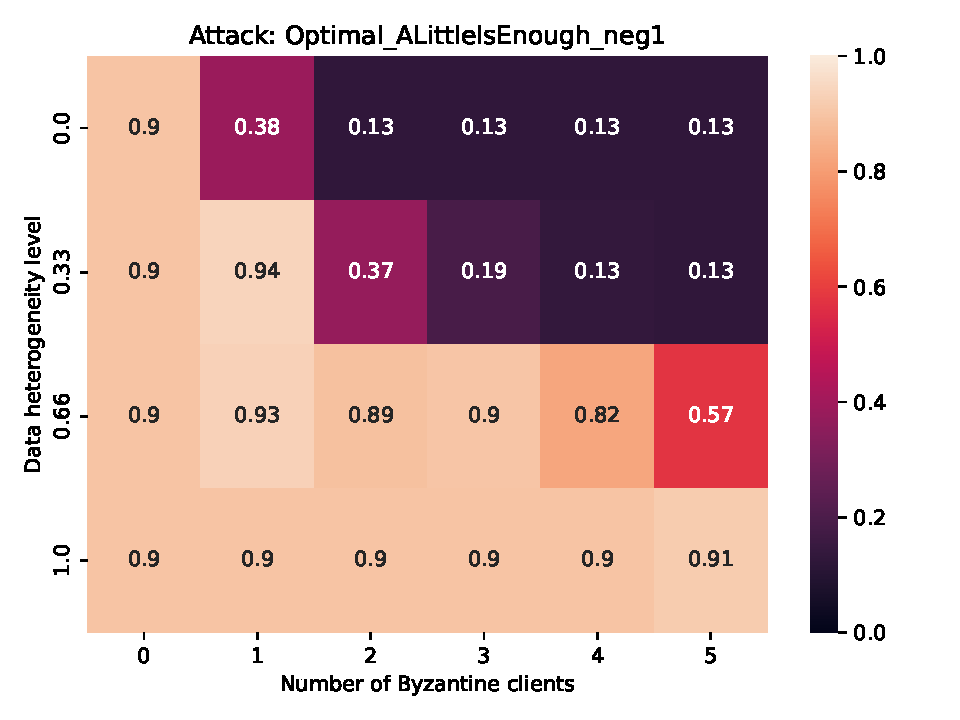
\includegraphics[width=\textwidth]{heatmap_tri_beta_0_75_optalie.pdf}
        \caption{$\beta = 0.75$}
        \label{fig:beta_0_75_optalie}
    \end{subfigure}
    \hfill
    \begin{subfigure}[b]{0.32\textwidth}
        \centering
        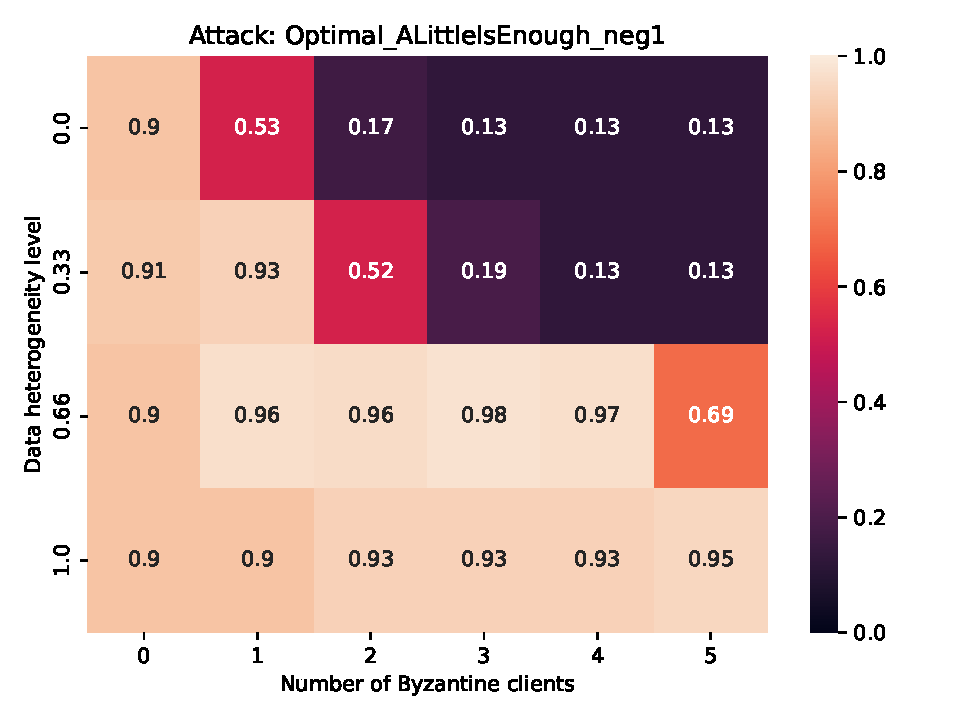
\includegraphics[width=\textwidth]{heatmap_tri_beta_1_0_optalie.pdf}
        \caption{$\beta = 1.0$}
        \label{fig:beta_1_0_optalie}
    \end{subfigure}
    
    \vspace{0.4cm}
    
    \begin{subfigure}[b]{0.32\textwidth}
        \centering
        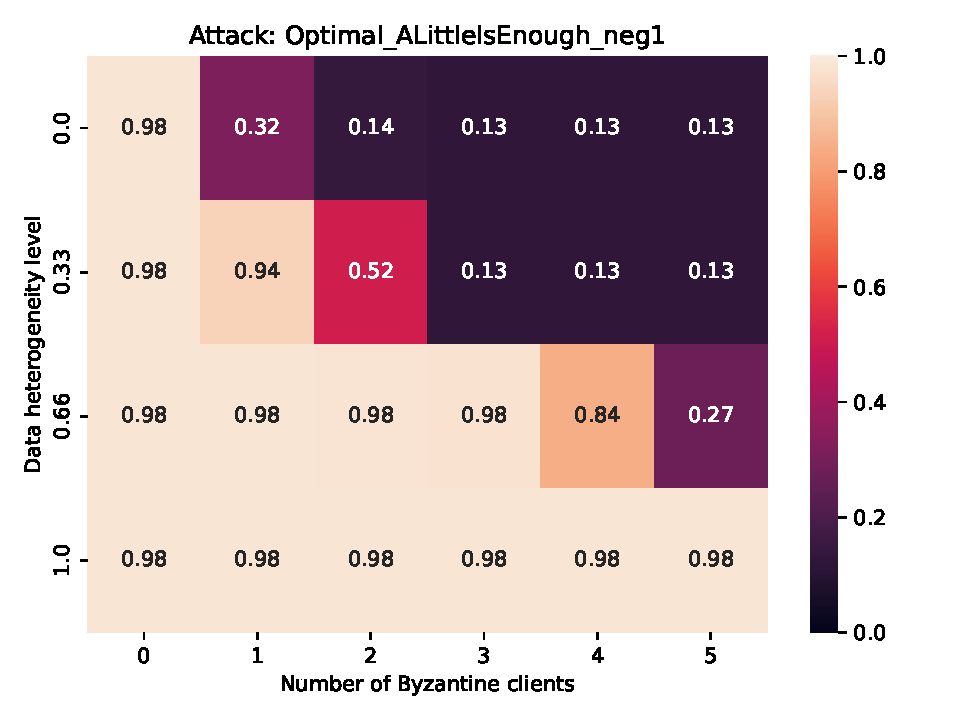
\includegraphics[width=\textwidth]{heatmap_tri_beta_1_25_optalie.pdf}
        \caption{$\beta = 1.25$}
        \label{fig:beta_1_25_optalie}
    \end{subfigure}
    \hfill
    \begin{subfigure}[b]{0.32\textwidth}
        \centering
        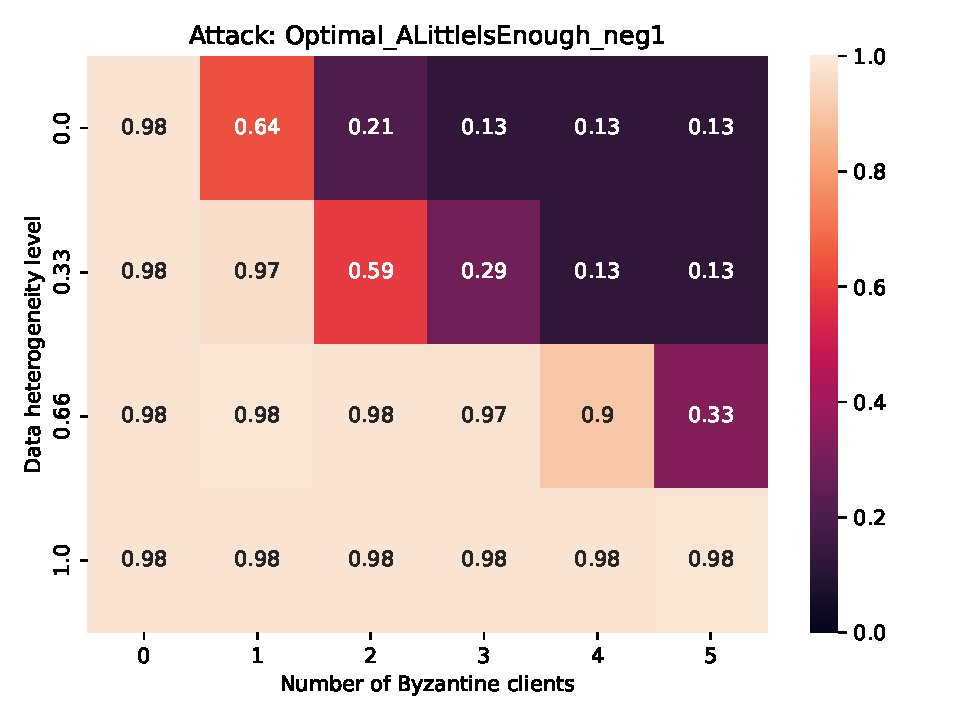
\includegraphics[width=\textwidth]{heatmap_tri_beta_1_5_optalie.pdf}
        \caption{$\beta = 1.5$}
        \label{fig:beta_1_5_optalie}
    \end{subfigure}
    \hfill
    \begin{subfigure}[b]{0.32\textwidth}
        \centering
        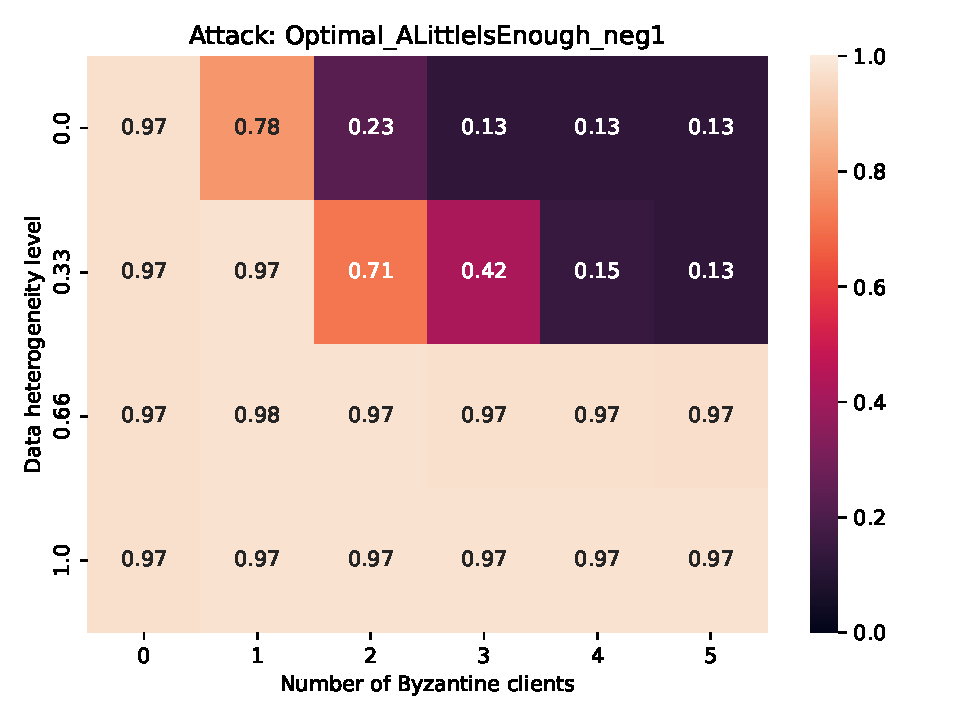
\includegraphics[width=\textwidth]{heatmap_tri_beta_2_0_optalie.pdf}
        \caption{$\beta = 2.0$}
        \label{fig:beta_2_0_optalie}
    \end{subfigure}
    
    \caption{Triangular (\texttt{tri}) comparison under Optimal ALIE attack for $\beta \in \{0.5, 0.75, 1.0, 1.25, 1.5, 2.0\}$.}
    \label{fig:tri_comparison_optalie}
\end{figure}

\clearpage

\subsection{Sign Flipping Attack}
The figure below displays the best test accuracy heatmaps under the Sign Flipping attack for different $\beta$ values of the Triangular surrogate gradient.

\begin{figure}[htbp]
    \centering
    \begin{subfigure}[b]{0.32\textwidth}
        \centering
        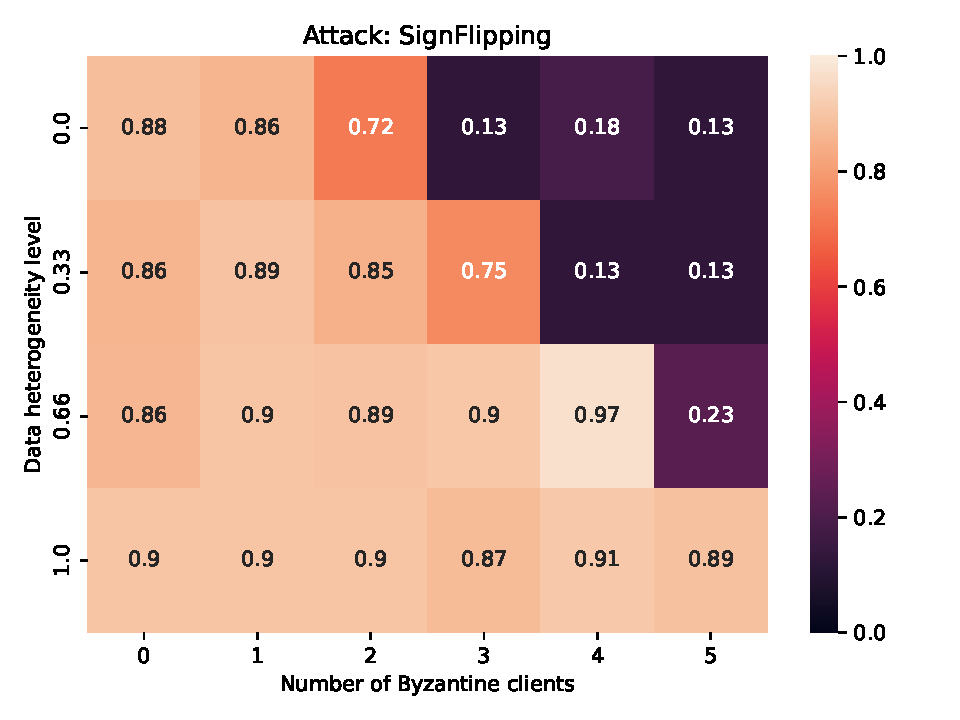
\includegraphics[width=\textwidth]{heatmap_tri_beta_0_5_sf.pdf}
        \caption{$\beta = 0.5$}
        \label{fig:beta_0_5_sf}
    \end{subfigure}
    \hfill
    \begin{subfigure}[b]{0.32\textwidth}
        \centering
        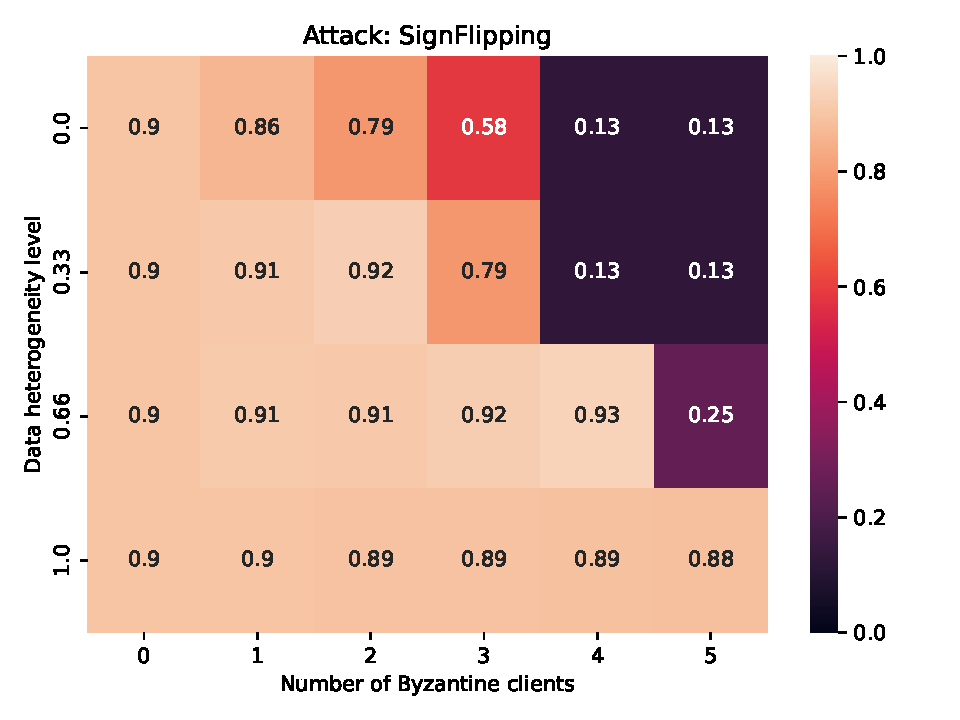
\includegraphics[width=\textwidth]{heatmap_tri_beta_0_75_sf.pdf}
        \caption{$\beta = 0.75$}
        \label{fig:beta_0_75_sf}
    \end{subfigure}
    \hfill
    \begin{subfigure}[b]{0.32\textwidth}
        \centering
        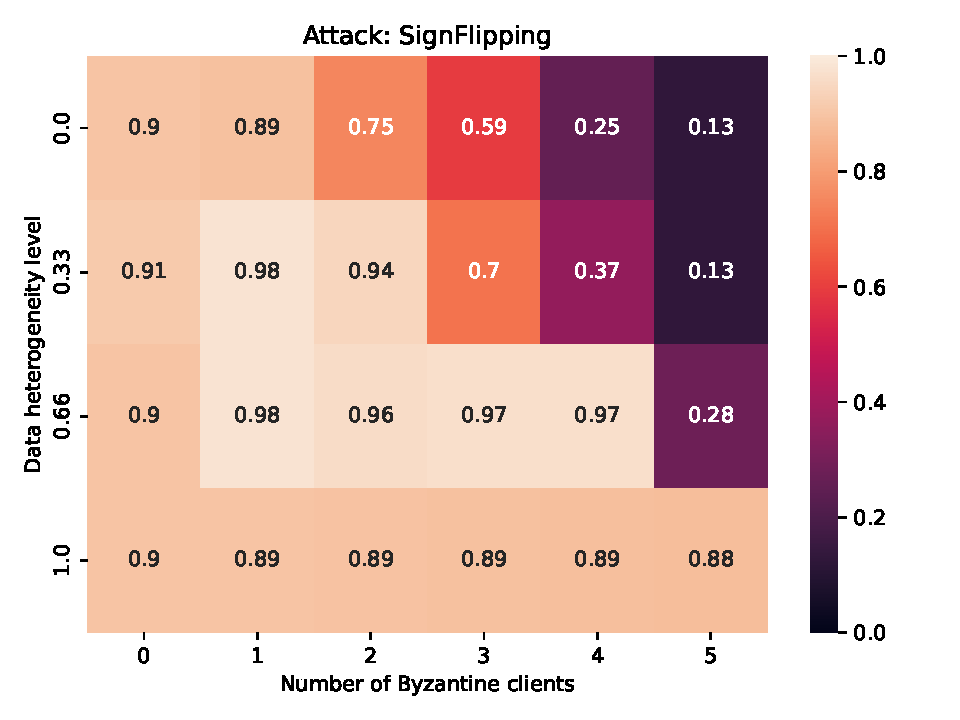
\includegraphics[width=\textwidth]{heatmap_tri_beta_1_0_sf.pdf}
        \caption{$\beta = 1.0$}
        \label{fig:beta_1_0_sf}
    \end{subfigure}
    
    \vspace{0.4cm}
    
    \begin{subfigure}[b]{0.32\textwidth}
        \centering
        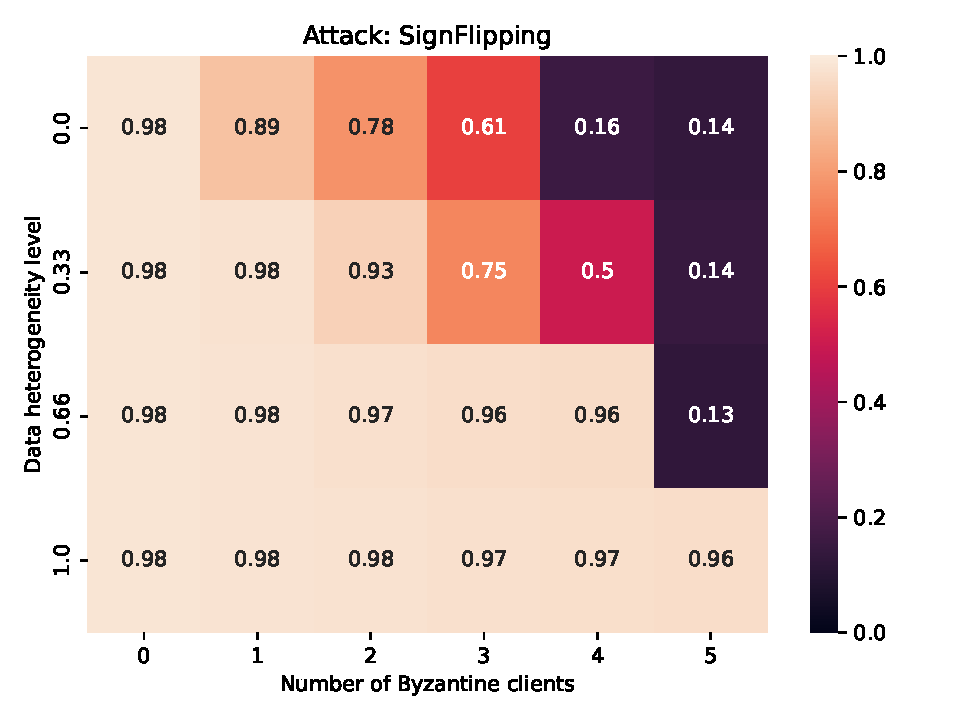
\includegraphics[width=\textwidth]{heatmap_tri_beta_1_25_sf.pdf}
        \caption{$\beta = 1.25$}
        \label{fig:beta_1_25_sf}
    \end{subfigure}
    \hfill
    \begin{subfigure}[b]{0.32\textwidth}
        \centering
        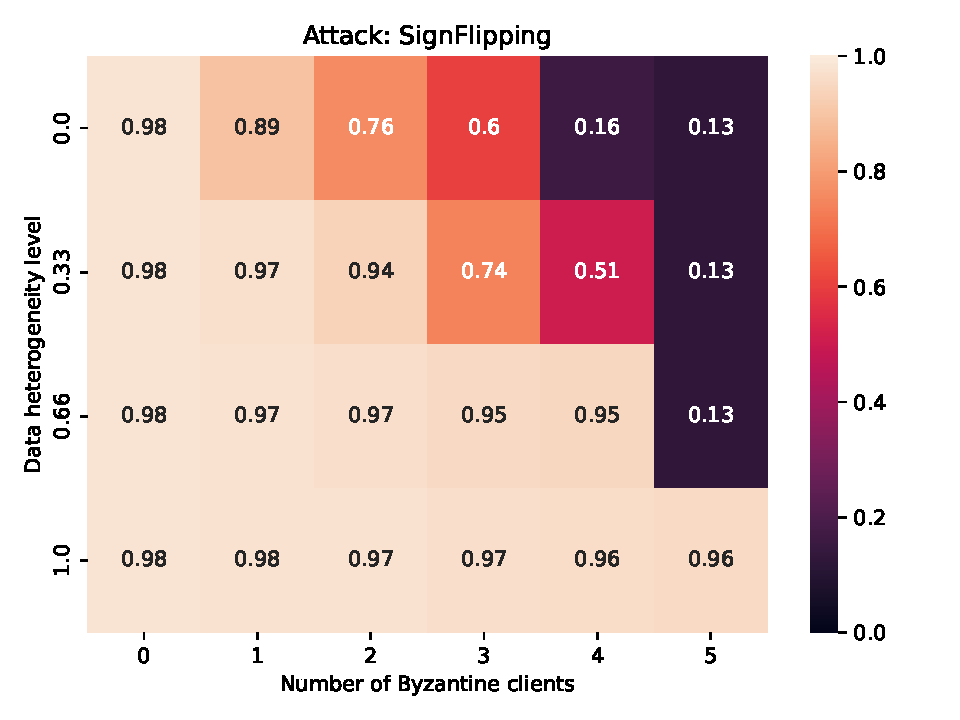
\includegraphics[width=\textwidth]{heatmap_tri_beta_1_5_sf.pdf}
        \caption{$\beta = 1.5$}
        \label{fig:beta_1_5_sf}
    \end{subfigure}
    \hfill
    \begin{subfigure}[b]{0.32\textwidth}
        \centering
        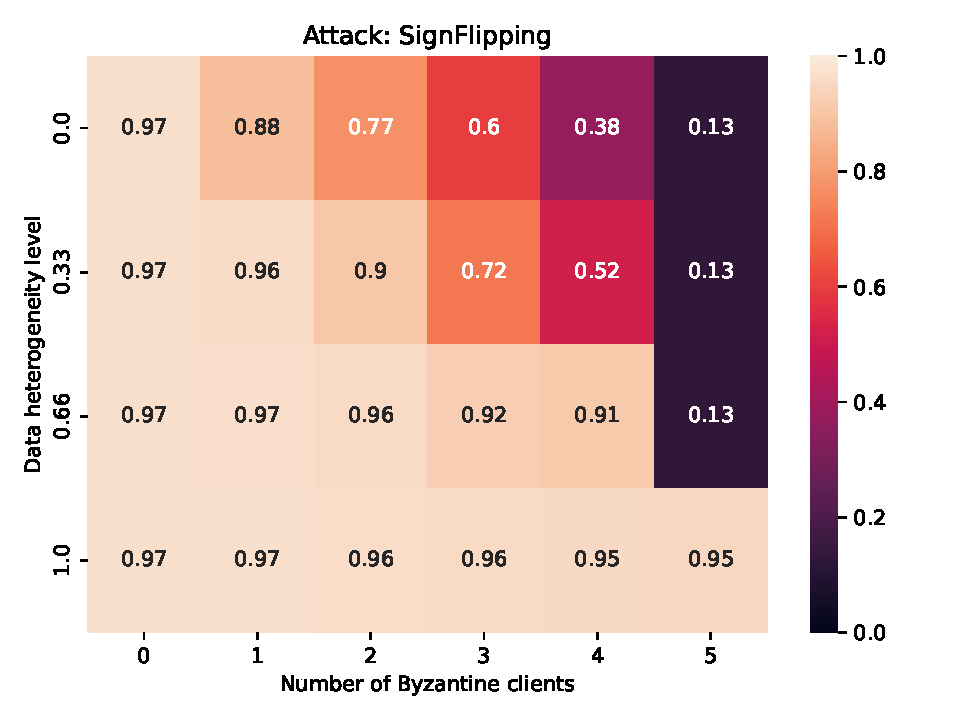
\includegraphics[width=\textwidth]{heatmap_tri_beta_2_0_sf.pdf}
        \caption{$\beta = 2.0$}
        \label{fig:beta_2_0_sf}
    \end{subfigure}
    
    \caption{Triangular (\texttt{tri}) comparison under Sign Flipping attack for $\beta \in \{0.5, 0.75, 1.0, 1.25, 1.5, 2.0\}$.}
    \label{fig:tri_comparison_sf}
\end{figure}

\clearpage

\section{Box (\texttt{box}) Surrogate Gradient stiffness sweeps}

\subsection{Best Overall Aggregator (Worst-Case Across Attacks)}
The figure below displays the test accuracy heatmaps under the worst-case attack scenario for different $\beta$ values of the Box surrogate gradient.

\begin{figure}[htbp]
    \centering
    \begin{subfigure}[b]{0.32\textwidth}
        \centering
        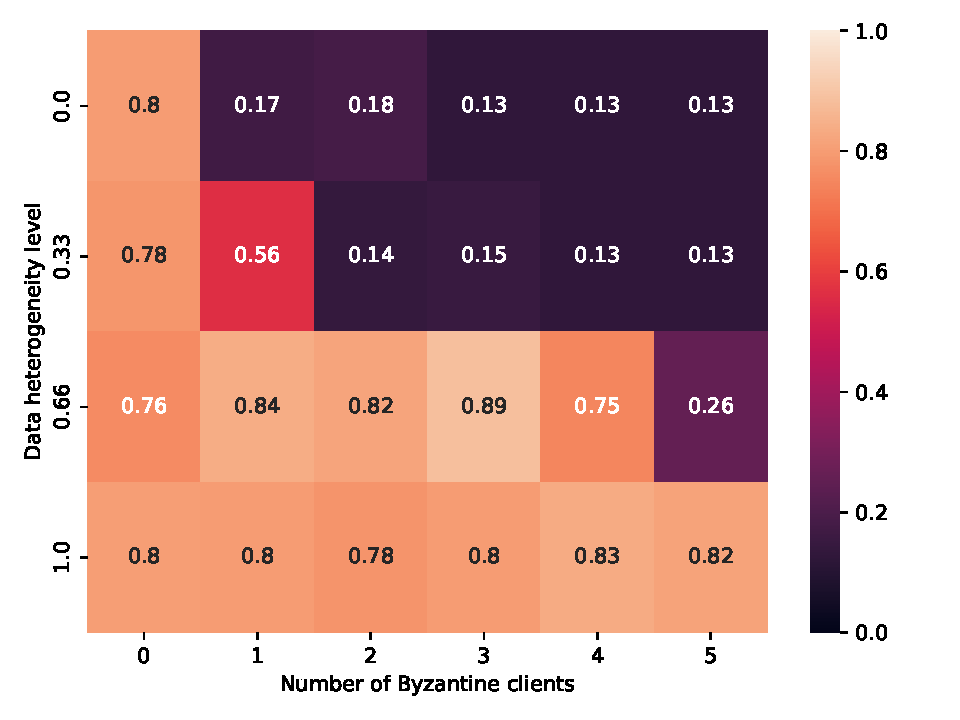
\includegraphics[width=\textwidth]{heatmap_box_beta_0_25_best.pdf}
        \caption{$\beta = 0.25$}
        \label{fig:box_beta_0_25_best}
    \end{subfigure}
    \hfill
    \begin{subfigure}[b]{0.32\textwidth}
        \centering
        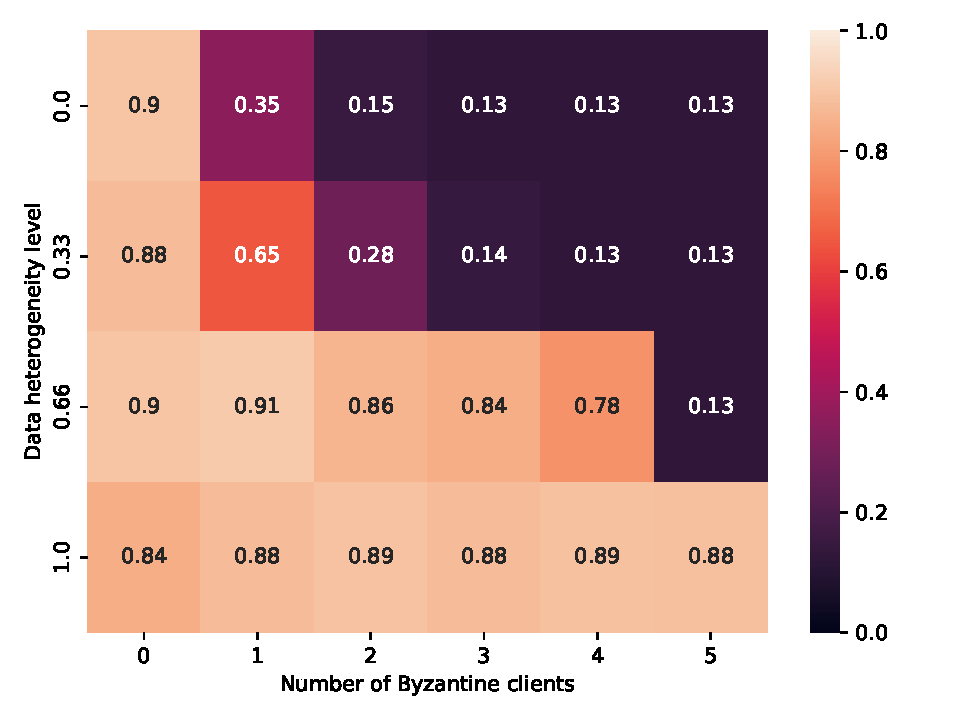
\includegraphics[width=\textwidth]{heatmap_box_beta_0_5_best.pdf}
        \caption{$\beta = 0.5$}
        \label{fig:box_beta_0_5_best}
    \end{subfigure}
    \hfill
    \begin{subfigure}[b]{0.32\textwidth}
        \centering
        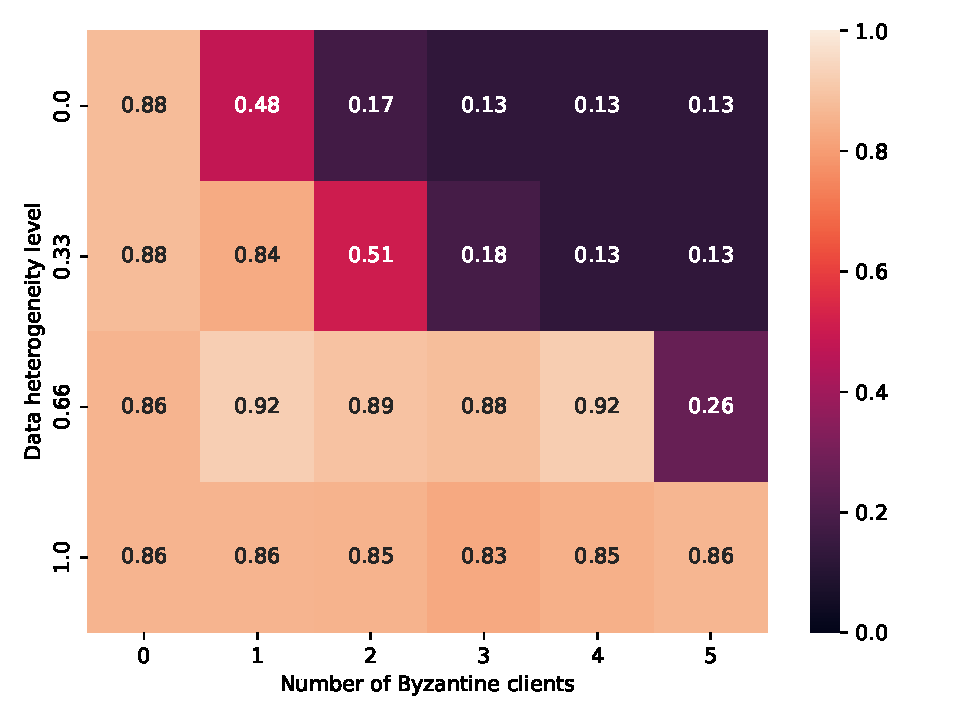
\includegraphics[width=\textwidth]{heatmap_box_beta_0_75_best.pdf}
        \caption{$\beta = 0.75$}
        \label{fig:box_beta_0_75_best}
    \end{subfigure}
    
    \vspace{0.4cm}
    
    \begin{subfigure}[b]{0.32\textwidth}
        \centering
        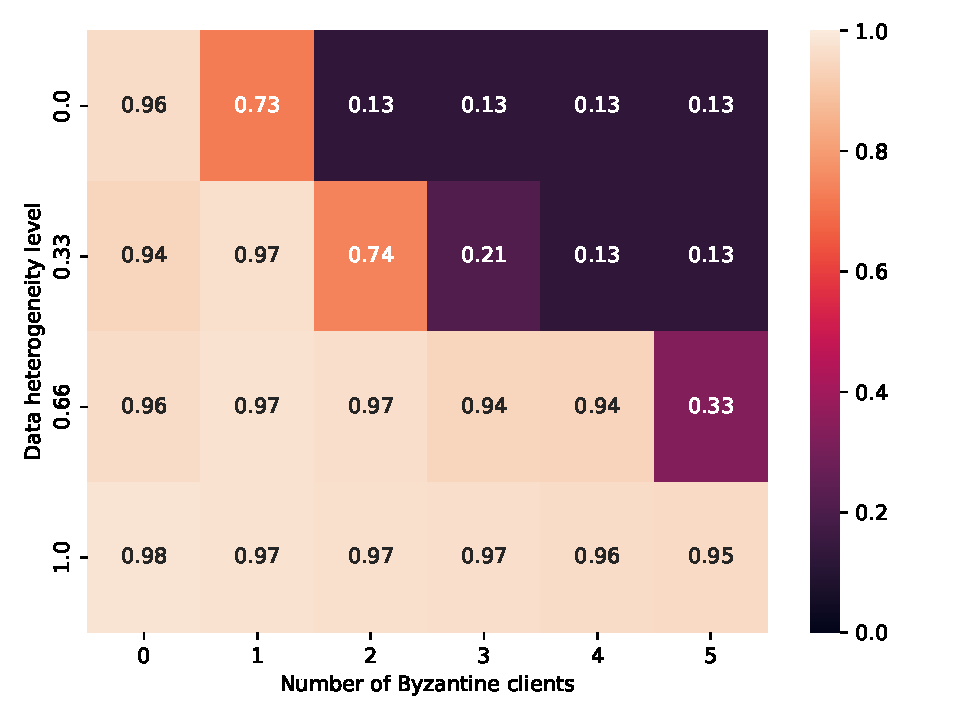
\includegraphics[width=\textwidth]{heatmap_box_beta_1_0_best.pdf}
        \caption{$\beta = 1.0$}
        \label{fig:box_beta_1_0_best}
    \end{subfigure}
    \hfill
    \begin{subfigure}[b]{0.32\textwidth}
        \centering
        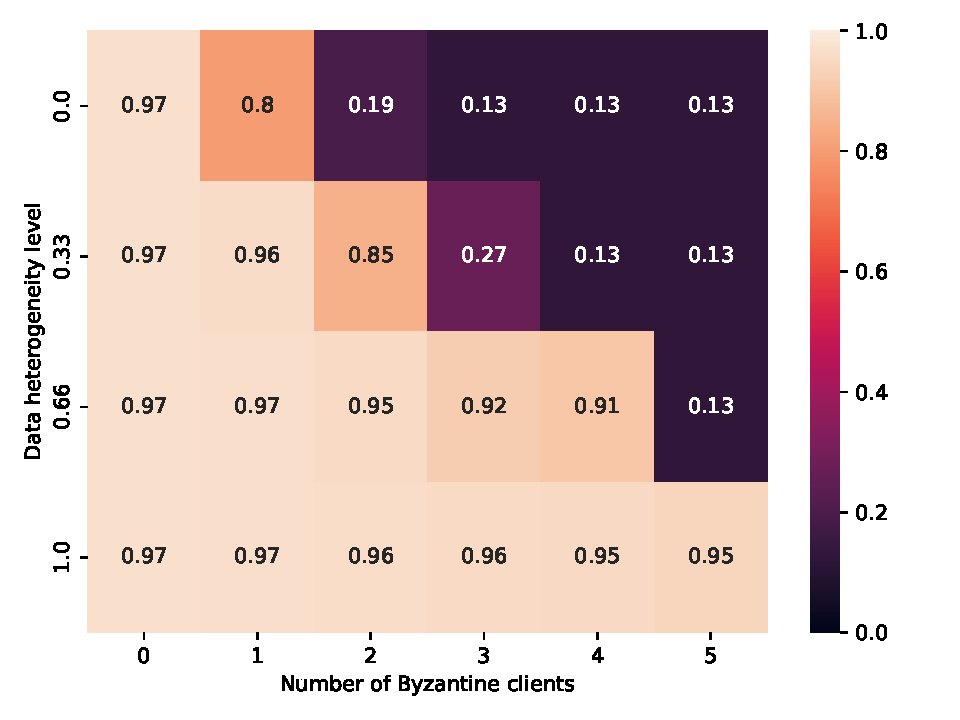
\includegraphics[width=\textwidth]{heatmap_box_beta_1_25_best.pdf}
        \caption{$\beta = 1.25$}
        \label{fig:box_beta_1_25_best}
    \end{subfigure}
    \hfill
    \begin{subfigure}[b]{0.32\textwidth}
        \centering
        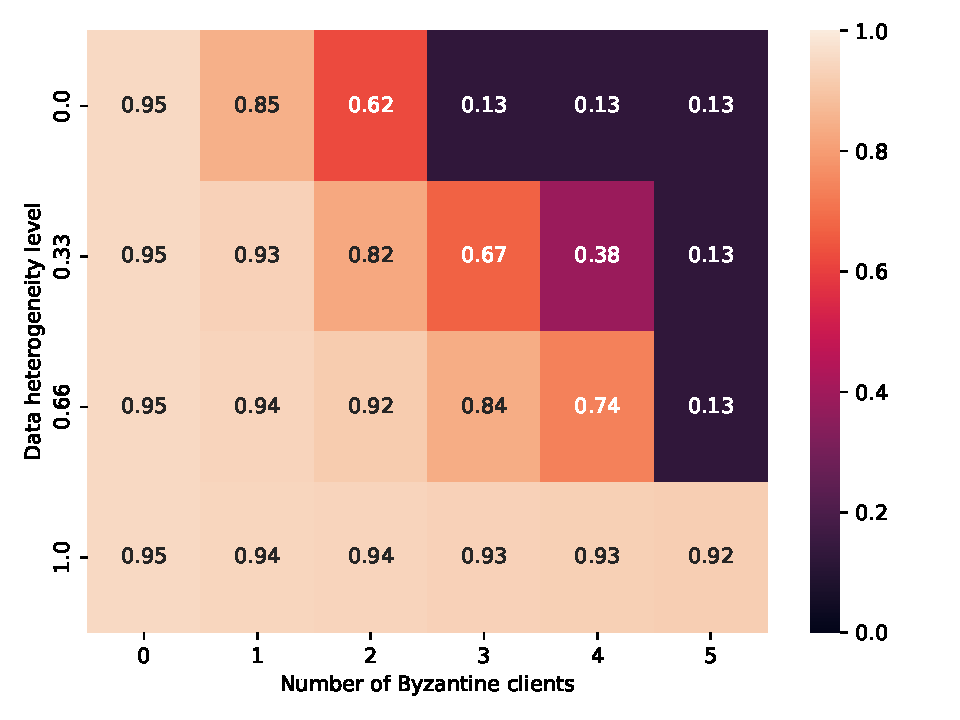
\includegraphics[width=\textwidth]{heatmap_box_beta_2_0_best.pdf}
        \caption{$\beta = 2.0$}
        \label{fig:box_beta_2_0_best}
    \end{subfigure}
    
    \caption{Box (\texttt{box}) comparison for best overall aggregator (worst-case) for $\beta \in \{0.25, 0.5, 0.75, 1.0, 1.25, 2.0\}$.}
    \label{fig:box_comparison_best}
\end{figure}

\clearpage

\subsection{Optimal ALIE Attack}
The figure below displays the best test accuracy heatmaps under the Optimal ALIE attack for different $\beta$ values of the Box surrogate gradient.

\begin{figure}[htbp]
    \centering
    \begin{subfigure}[b]{0.32\textwidth}
        \centering
        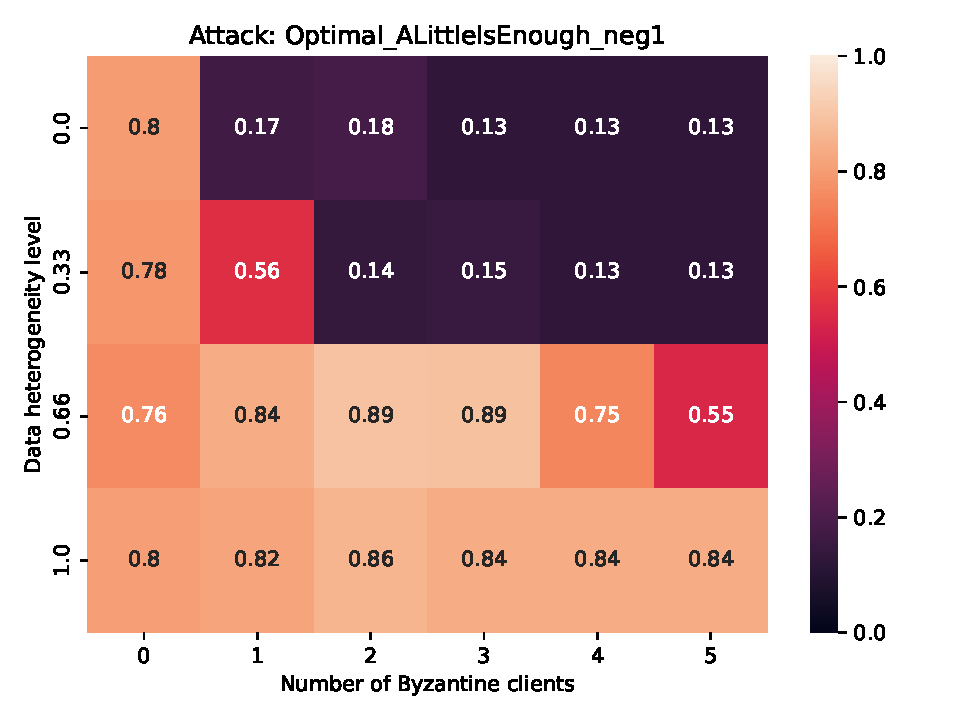
\includegraphics[width=\textwidth]{heatmap_box_beta_0_25_optalie.pdf}
        \caption{$\beta = 0.25$}
        \label{fig:box_beta_0_25_optalie}
    \end{subfigure}
    \hfill
    \begin{subfigure}[b]{0.32\textwidth}
        \centering
        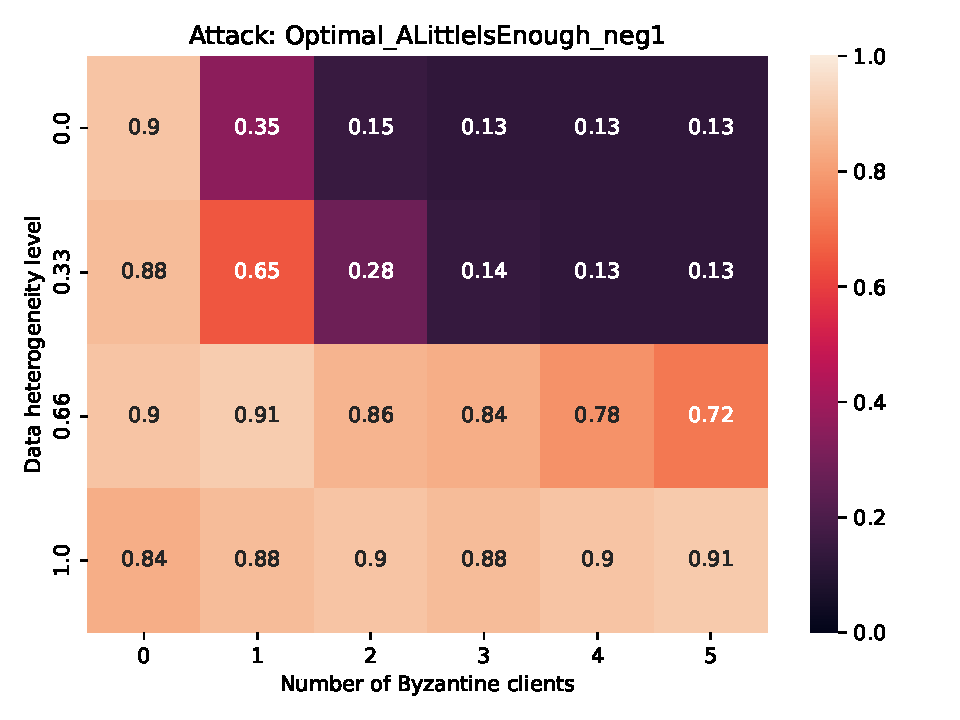
\includegraphics[width=\textwidth]{heatmap_box_beta_0_5_optalie.pdf}
        \caption{$\beta = 0.5$}
        \label{fig:box_beta_0_5_optalie}
    \end{subfigure}
    \hfill
    \begin{subfigure}[b]{0.32\textwidth}
        \centering
        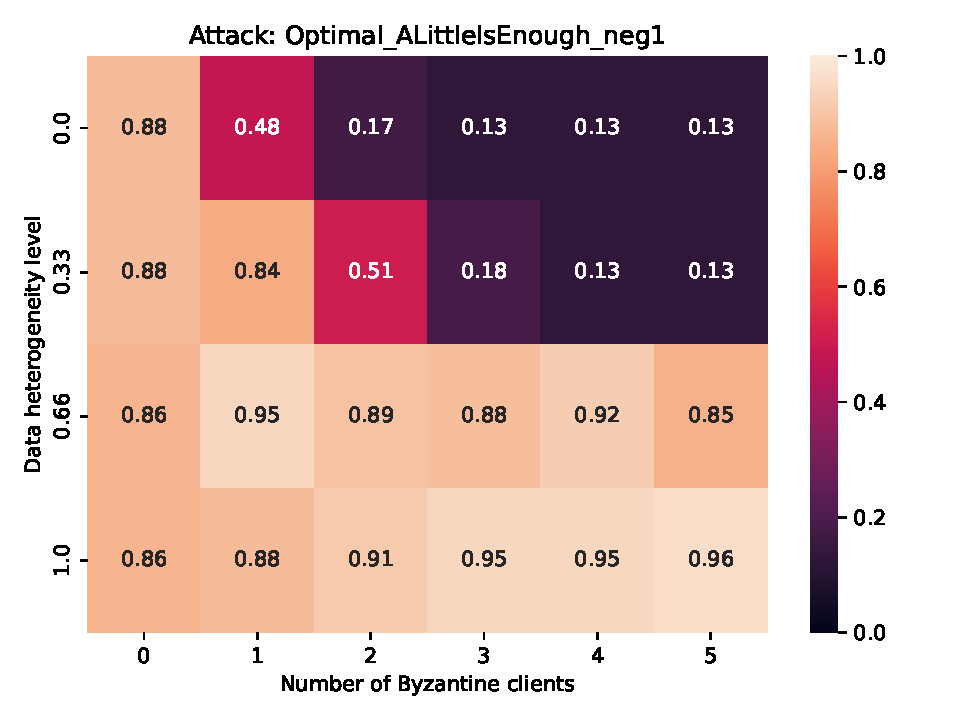
\includegraphics[width=\textwidth]{heatmap_box_beta_0_75_optalie.pdf}
        \caption{$\beta = 0.75$}
        \label{fig:box_beta_0_75_optalie}
    \end{subfigure}
    
    \vspace{0.4cm}
    
    \begin{subfigure}[b]{0.32\textwidth}
        \centering
        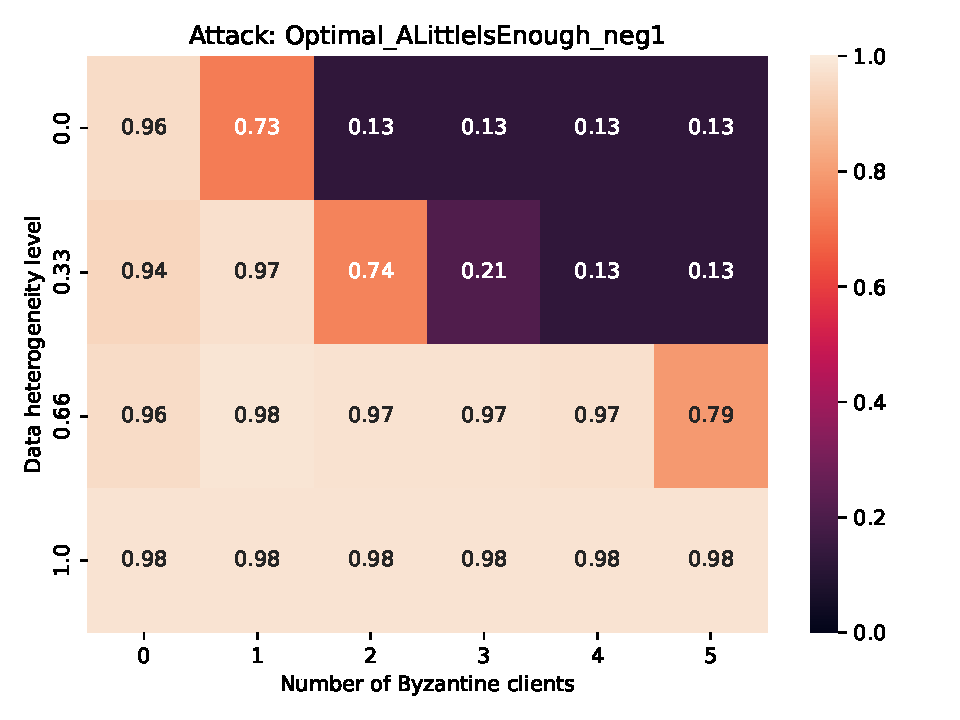
\includegraphics[width=\textwidth]{heatmap_box_beta_1_0_optalie.pdf}
        \caption{$\beta = 1.0$}
        \label{fig:box_beta_1_0_optalie}
    \end{subfigure}
    \hfill
    \begin{subfigure}[b]{0.32\textwidth}
        \centering
        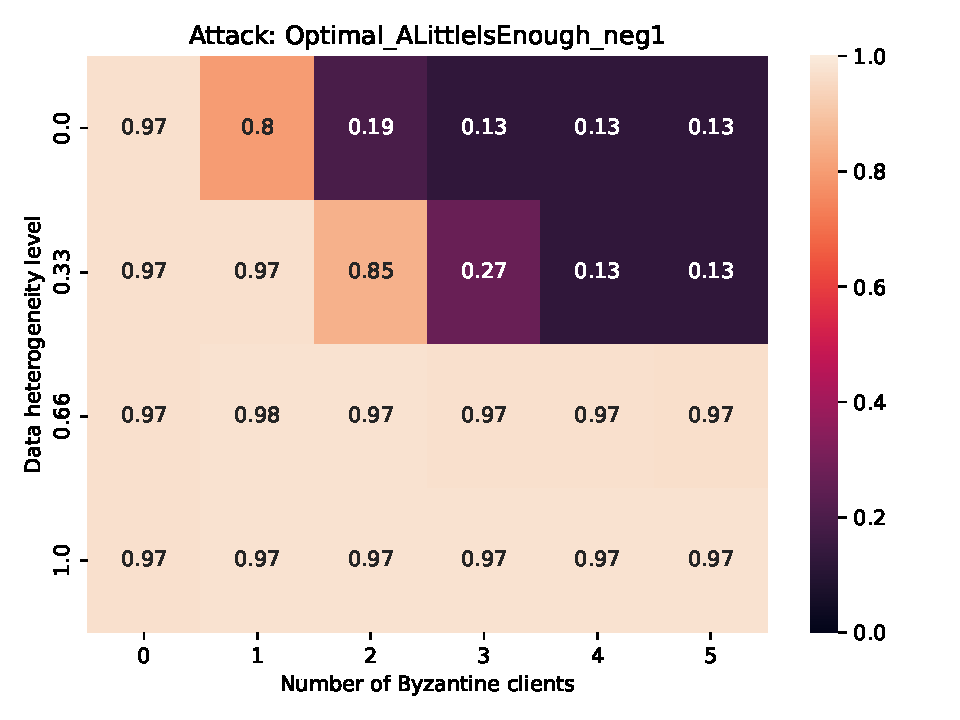
\includegraphics[width=\textwidth]{heatmap_box_beta_1_25_optalie.pdf}
        \caption{$\beta = 1.25$}
        \label{fig:box_beta_1_25_optalie}
    \end{subfigure}
    \hfill
    \begin{subfigure}[b]{0.32\textwidth}
        \centering
        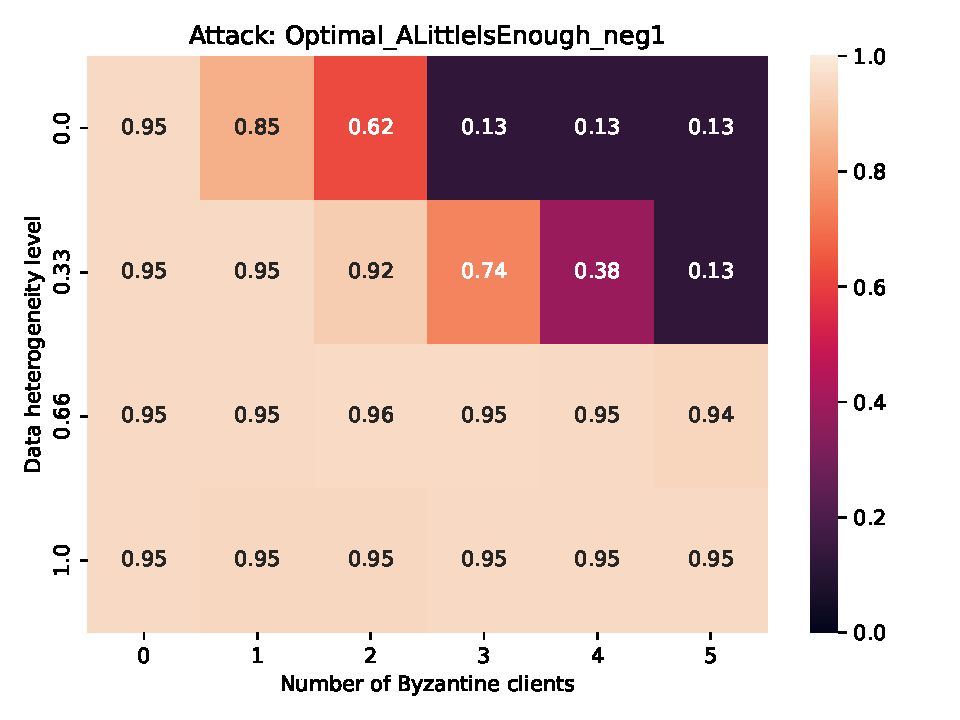
\includegraphics[width=\textwidth]{heatmap_box_beta_2_0_optalie.pdf}
        \caption{$\beta = 2.0$}
        \label{fig:box_beta_2_0_optalie}
    \end{subfigure}
    
    \caption{Box (\texttt{box}) comparison under Optimal ALIE attack for $\beta \in \{0.25, 0.5, 0.75, 1.0, 1.25, 2.0\}$.}
    \label{fig:box_comparison_optalie}
\end{figure}

\clearpage

\subsection{Sign Flipping Attack}
The figure below displays the best test accuracy heatmaps under the Sign Flipping attack for different $\beta$ values of the Box surrogate gradient.

\begin{figure}[htbp]
    \centering
    \begin{subfigure}[b]{0.32\textwidth}
        \centering
        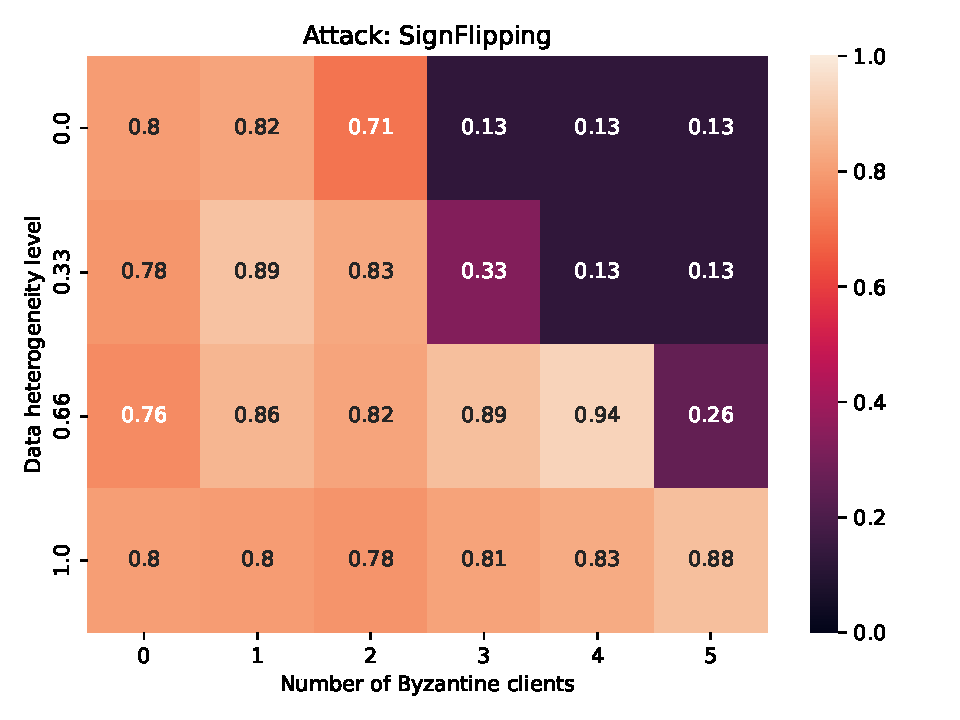
\includegraphics[width=\textwidth]{heatmap_box_beta_0_25_sf.pdf}
        \caption{$\beta = 0.25$}
        \label{fig:box_beta_0_25_sf}
    \end{subfigure}
    \hfill
    \begin{subfigure}[b]{0.32\textwidth}
        \centering
        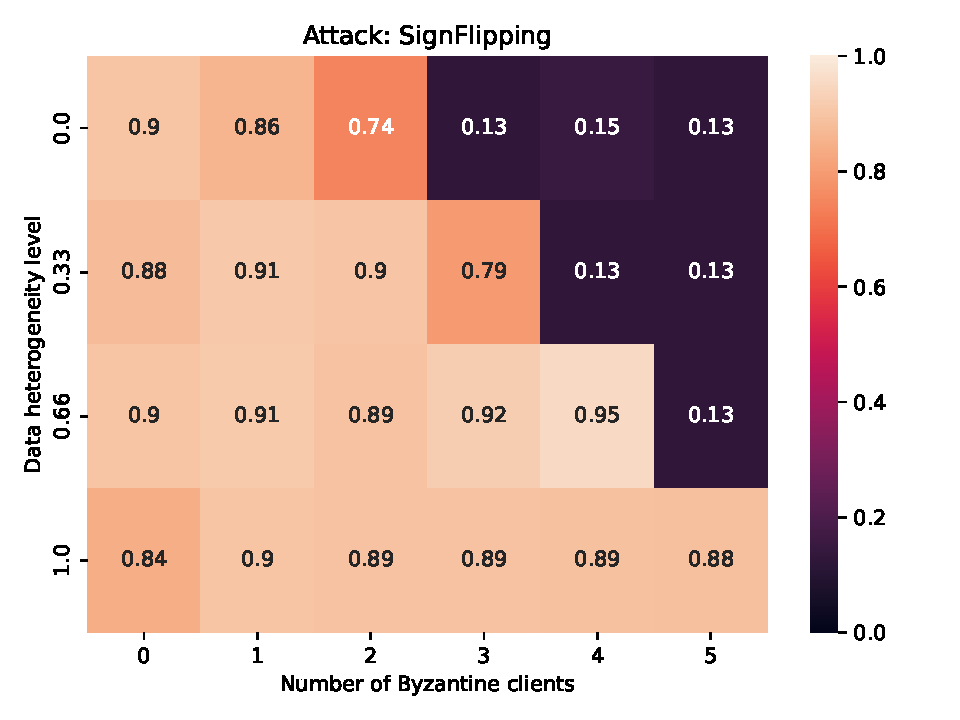
\includegraphics[width=\textwidth]{heatmap_box_beta_0_5_sf.pdf}
        \caption{$\beta = 0.5$}
        \label{fig:box_beta_0_5_sf}
    \end{subfigure}
    \hfill
    \begin{subfigure}[b]{0.32\textwidth}
        \centering
        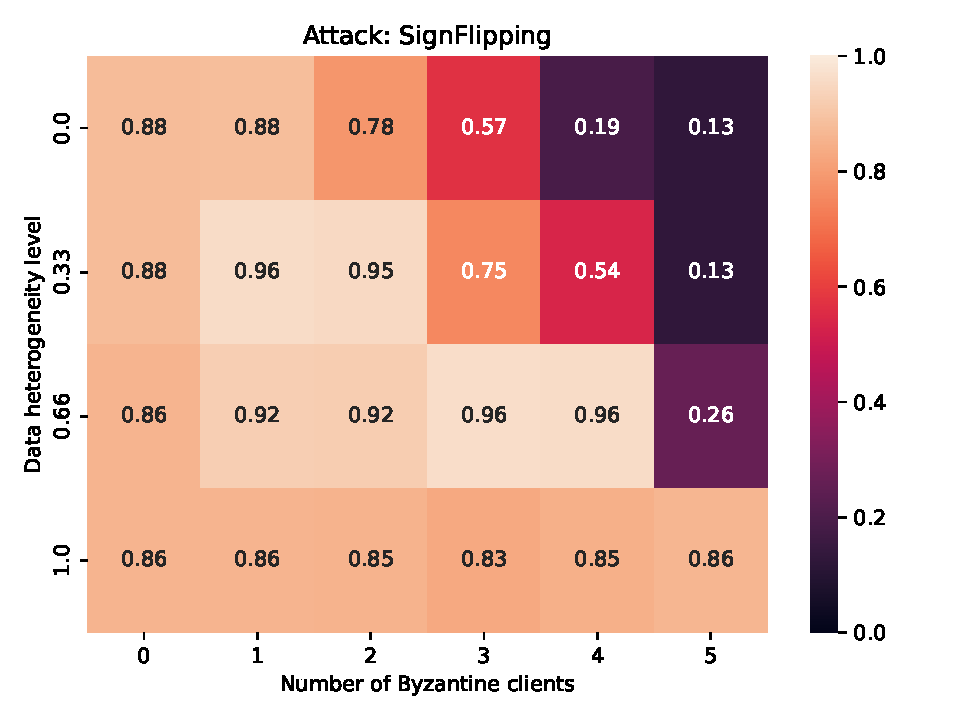
\includegraphics[width=\textwidth]{heatmap_box_beta_0_75_sf.pdf}
        \caption{$\beta = 0.75$}
        \label{fig:box_beta_0_75_sf}
    \end{subfigure}
    
    \vspace{0.4cm}
    
    \begin{subfigure}[b]{0.32\textwidth}
        \centering
        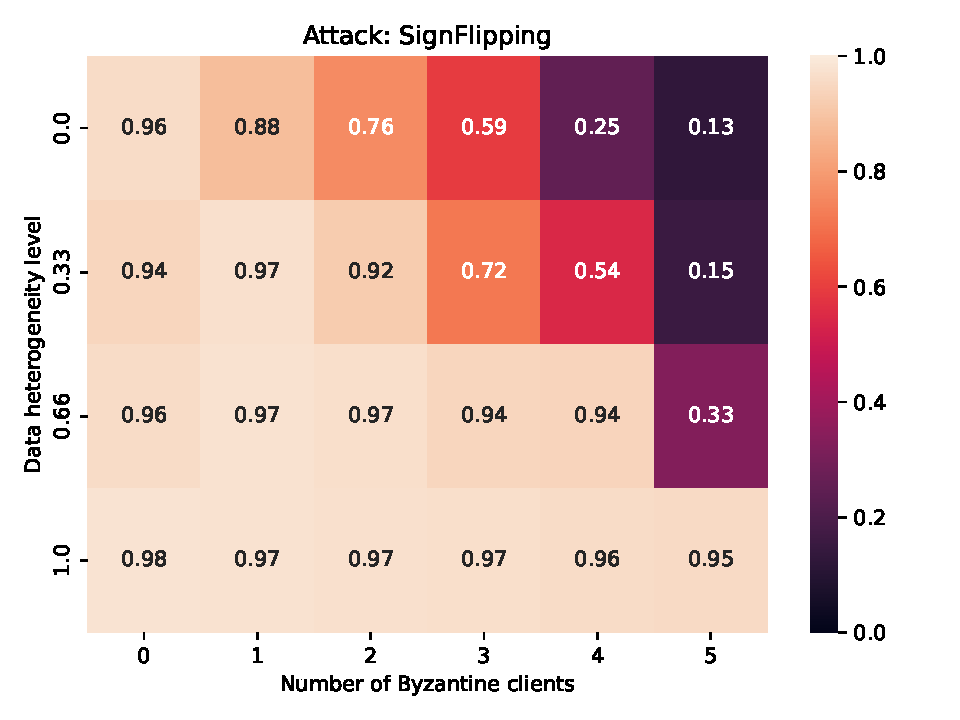
\includegraphics[width=\textwidth]{heatmap_box_beta_1_0_sf.pdf}
        \caption{$\beta = 1.0$}
        \label{fig:box_beta_1_0_sf}
    \end{subfigure}
    \hfill
    \begin{subfigure}[b]{0.32\textwidth}
        \centering
        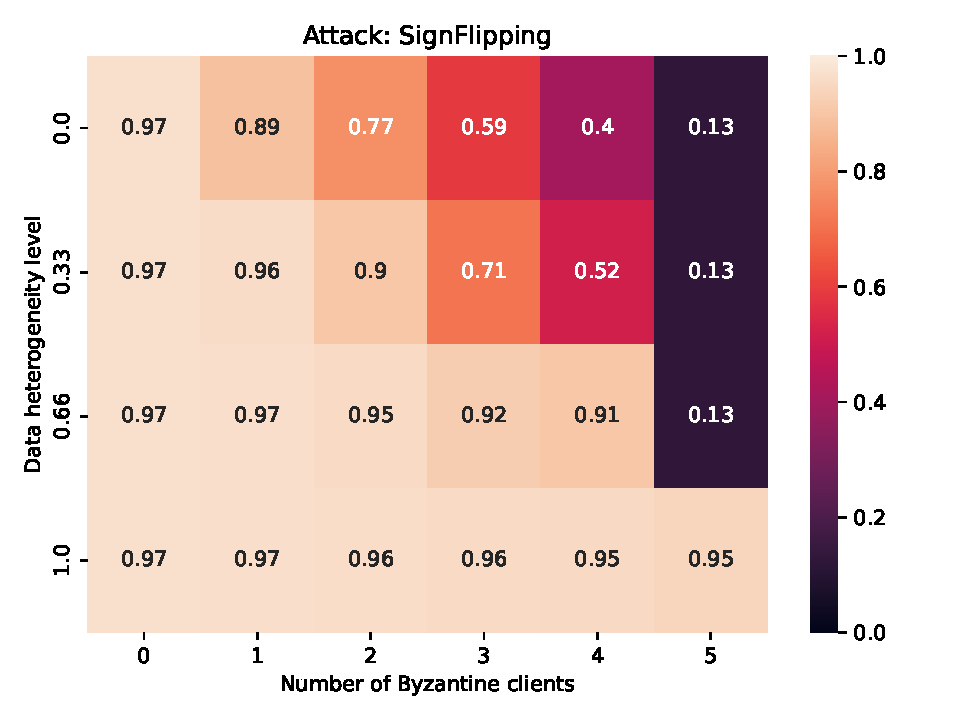
\includegraphics[width=\textwidth]{heatmap_box_beta_1_25_sf.pdf}
        \caption{$\beta = 1.25$}
        \label{fig:box_beta_1_25_sf}
    \end{subfigure}
    \hfill
    \begin{subfigure}[b]{0.32\textwidth}
        \centering
        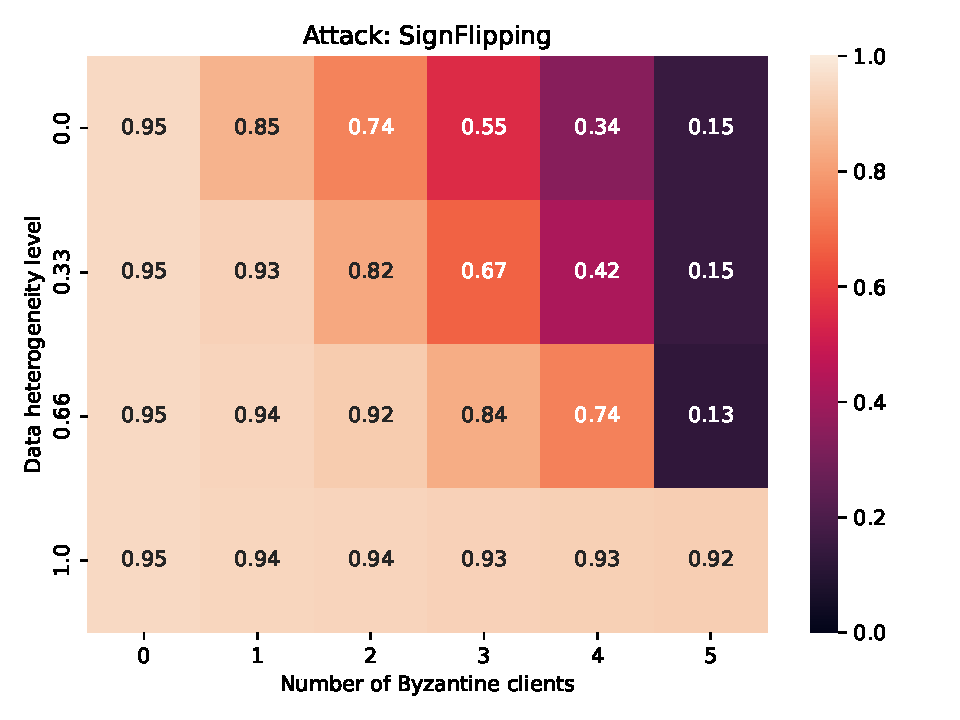
\includegraphics[width=\textwidth]{heatmap_box_beta_2_0_sf.pdf}
        \caption{$\beta = 2.0$}
        \label{fig:box_beta_2_0_sf}
    \end{subfigure}
    
    \caption{Box (\texttt{box}) comparison under Sign Flipping attack for $\beta \in \{0.25, 0.5, 0.75, 1.0, 1.25, 2.0\}$.}
    \label{fig:box_comparison_sf}
\end{figure}

\end{document}
